\section{Introduction}
%
The railway network is a complex and interconnected system that comprises a multitude of critical components, such as track circuits, switches, signals, and many others. All these elements work together to ensure the safe and efficient operation of the entire network. At the core of a railway infrastructure there are two systems: the \gls{is} and \gls{rbc}.

\begin{comment}
	The \gls{is} is responsible to ensure efficient and safe operation of the railway network monitoring and managing the status of all the railway elements, ensuring that they are functioning and communicating properly. By constantly monitoring the status of track circuits, switches, and all the railway elements,  is able to send commands to signal switches and other essential railway components. 
\end{comment}

The \gls{is} plays a crucial role in guaranteeing the efficient and safe operation of the railway network by continuously overseeing and managing the status of all its elements. It ensures their proper functioning and communication. Through real-time monitoring of track circuits, switches, and various railway components, the \gls{is} has the capability to issue commands to signal switches and other essential elements, thereby maintaining optimal railway functionality.

The second important element of the railway network is the \gls{rbc} which serves as the interface between the \gls{is} and the on-board trains. In Europe, it is based on \gls{ertms} a standardized and interoperable train control and command system for railways~\cite{ertms}. In its pursuit of ensuring the secure spacing of trains, the \gls{rbc} leverages real-time insights into the current state of the railway network. This comprehensive understanding is derived from the data received both from the \gls{is} and the dynamic information regarding the positions and velocities of actively circulating trains. The goal of the \gls{rbc} is to manage and optimize the safe distances between trains, thereby contributing to the overall safety and efficiency of railway operations. In this work, the \gls{rbc} will be considered the actor which is in charge to initiate a \gls{vc} operation between trains.
%
\begin{figure}[!ht]
	\resizebox{\linewidth}{!}{

\pgfplotsset{width=5cm,compat=1.18}

\tikzset{every picture/.style={line width=0.75pt}} %set default line width to 0.75pt        

\begin{tikzpicture}[x=0.75pt,y=0.75pt,yscale=-1,xscale=1]
%uncomment if require: \path (0,300); %set diagram left start at 0, and has height of 300

%Image [id:dp0011035212048724485] 
\draw (307.8,139.93) node  {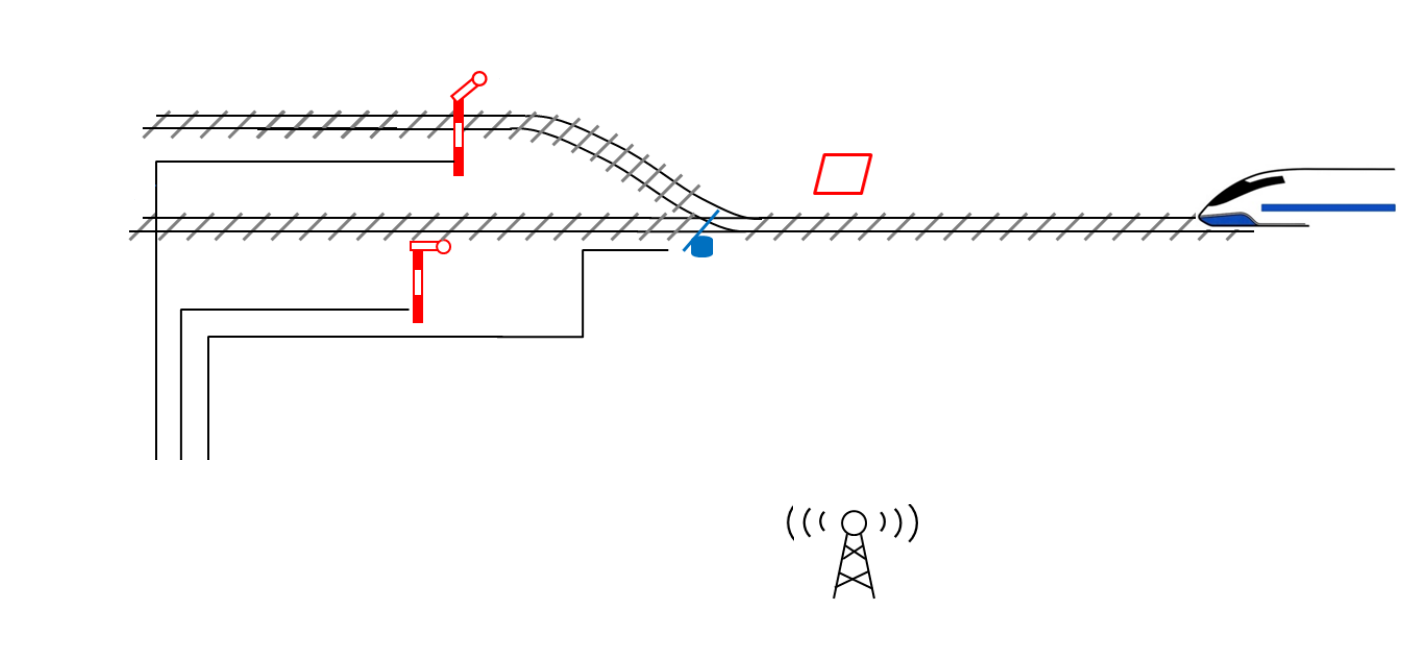
\includegraphics[width=350.8pt,height=176.4pt]{figure/railwayNetwork.png}};
%Rounded Rect [id:dp8635061097341326] 
\draw   (104.33,199.93) .. controls (104.33,192.79) and (110.12,187) .. (117.27,187) -- (156.07,187) .. controls (163.21,187) and (169,192.79) .. (169,199.93) -- (169,245.4) .. controls (169,252.54) and (163.21,258.33) .. (156.07,258.33) -- (117.27,258.33) .. controls (110.12,258.33) and (104.33,252.54) .. (104.33,245.4) -- cycle ;
%Right Arrow [id:dp5902707358380477] 
\draw   (169,199.93) -- (225.4,199.93) -- (225.4,191.7) -- (263,208.17) -- (225.4,224.63) -- (225.4,216.4) -- (169,216.4) -- cycle ;
%Rounded Rect [id:dp6848372643216789] 
\draw   (261.67,195.93) .. controls (261.67,188.79) and (267.46,183) .. (274.6,183) -- (313.4,183) .. controls (320.54,183) and (326.33,188.79) .. (326.33,195.93) -- (326.33,241.4) .. controls (326.33,248.54) and (320.54,254.33) .. (313.4,254.33) -- (274.6,254.33) .. controls (267.46,254.33) and (261.67,248.54) .. (261.67,241.4) -- cycle ;
%Right Arrow [id:dp00995349944529833] 
\draw   (261.74,249.63) -- (205.34,250.14) -- (205.42,258.37) -- (167.67,242.24) -- (205.12,225.44) -- (205.2,233.67) -- (261.59,233.17) -- cycle ;
%Right Arrow [id:dp13455094966677605] 
\draw   (369.29,188.62) -- (418.51,139.44) -- (412.87,133.8) -- (456.96,112.29) -- (435.42,156.36) -- (429.78,150.72) -- (380.57,199.9) -- cycle ;
%Right Arrow [id:dp26740738968744493] 
\draw   (488.46,128.23) -- (428.65,190.74) -- (434.41,196.25) -- (383.01,226.89) -- (411.36,174.2) -- (417.12,179.71) -- (476.94,117.21) -- cycle ;

% Text Node
\draw    (238.6,28.4) -- (277.6,28.4) -- (277.6,49.4) -- (238.6,49.4) -- cycle  ;
\draw (239.6,29.4) node [anchor=north west][inner sep=0.75pt]  [font=\footnotesize] [align=left] {signal};
% Text Node
\draw    (364.6,37.73) -- (404.6,37.73) -- (404.6,75.73) -- (364.6,75.73) -- cycle  ;
\draw (365.6,38.73) node [anchor=north west][inner sep=0.75pt]  [font=\footnotesize] [align=left] {virtual\\signal};
% Text Node
\draw    (311.93,111.07) -- (352.93,111.07) -- (352.93,132.07) -- (311.93,132.07) -- cycle  ;
\draw (312.93,112.07) node [anchor=north west][inner sep=0.75pt]  [font=\footnotesize] [align=left] {switch};
% Text Node
\draw    (123.27,32.4) -- (192.27,32.4) -- (192.27,53.4) -- (123.27,53.4) -- cycle  ;
\draw (124.27,33.4) node [anchor=north west][inner sep=0.75pt]  [font=\footnotesize] [align=left] {track circuit};
% Text Node
\draw    (149.27,147.73) -- (192.27,147.73) -- (192.27,168.73) -- (149.27,168.73) -- cycle  ;
\draw (150.27,148.73) node [anchor=north west][inner sep=0.75pt]  [font=\footnotesize] [align=left] {cables};
% Text Node
\draw (115.33,211.33) node [anchor=north west][inner sep=0.75pt]   [align=left] {IS};
% Text Node
\draw (274.67,209.33) node [anchor=north west][inner sep=0.75pt]   [align=left] {RBC};
% Text Node
\draw (169,199.93) node [anchor=north west][inner sep=0.75pt]  [font=\footnotesize] [align=left] {element states};
% Text Node
\draw (190.67,232) node [anchor=north west][inner sep=0.75pt]  [font=\footnotesize] [align=left] {train data};
% Text Node
\draw (365.02,188.71) node [anchor=north west][inner sep=0.75pt]  [font=\footnotesize,rotate=-315.58] [align=left] {movement authority\\};
% Text Node
\draw (387.02,206.04) node [anchor=north west][inner sep=0.75pt]  [font=\footnotesize,rotate=-315.58] [align=left] {position, track requests\\};


\end{tikzpicture}


}
	\caption{Railway network.}
	\label{fig:railwayNetwork}
\end{figure}
%

To better understand the structure and complexity of the railway network, Figure \ref{fig:railwayNetwork} illustrates the various components and their interconnections. As the latter demonstrates, the \gls{is} is the core of the entire system, with all the railway elements and the \gls{rbc} connected to it. This allows for centralized control and real-time monitoring of the entire network, ensuring the safe and efficient operation of the railway system.

The current communication technology present on the railway infrastructure is \gls{v2i}, namely, the communication between the \gls{rbc} and trains. The existing standard \gls{v2i} is an integral component of the railway communication infrastructure, relying on the GSM-R network. Nowadays, the emergence of the 5G network-based railway communication technology, known as Future Railway Communication and Management System\cite{frmcs}, it is a viable \gls{v2v} technology which is gradually gaining prominence due to its advanced capabilities in data transfer, reliability and  low-latency characteristics, ensuring swift and real-time data exchange among trains within the network.

\begin{comment}
	The \gls{ertms} system relies on a specific language to convey information through various channels such as radio, balise, and loop airgaps. This language is comprised of several elements, including variables, packets, messages, and telegrams. Variables are used to encode single data values and cannot be divided into minor units. Each variable has a unique name and is associated with a specific meaning as defined in the variable definition. When multiple variables need to be grouped together, they are organized into packets. These packets have a defined internal structure, consisting of a packet header with unique packet numbers, packet lengths, orientation information, distance scales, and an information section containing a set of variables.
\end{comment}

The growing popularity of trains as a mode of transportation presents a challenge of overburdening the railway system's capacity. As a result, enhancing infrastructure utilization and increasing capacity are two crucial objectives that railways are currently striving to achieve. These goals are being tackled by Shift2Rail~\cite{shift2rail}, an initiative focused on developing innovative technologies and solutions to enhance the efficiency, safety, and sustainability of the railway system.

\begin{comment}
	The CCS TSI (Command Control and Signalling - Technical Specification for Interoperability) has already defined \gls{l3}, and operational applications of the system already exist. \gls{l3}, as specified by the CCS TSI Subset-026~\cite{subset026}, is a train control system that utilizes radio communication to generate \glspl{ma} trackside and transmit them to the train via Euroradio communication protocol; moreover, provides continuous speed supervision to prevent any potential overrun of the authority~\cite{l3}.
\end{comment}


In the following, we will introduce two \gls{ertms} technology standards, upon which the work is based: \gls{l3} and \gls{vc} which are depicted in Figure~\ref{fig:ertmsl3vc}.
By transitioning from fixed to virtual block systems, \gls{l3} reduces dependence on trackside signals and infrastructure, relying instead on advanced onboard systems and continuous  communication. This shift not only promises to enhance line capacity but also to reduce operational costs by optimizing train headways and minimizing the need for trackside maintenance; furthermore, it allows trains to move dynamically within a virtual continuously updated block which is is contingent upon the position of the preceding train~\cite{ertmsl3}.  


Nowadays, the technology for \gls{vc} is still in the conception stage, and research is underway to determine the best way to implement it~\cite{flamini2018}. The control field is particularly interested in finding a solution that can provide the necessary speed, reliability, and safety to support real-time communication between trains. In addition to these technical considerations, research in the control field is also underway to determine the best way to implement \gls{vc} from an operational perspective~\cite{dimeo2020}. This involves studying the impact of the new technology on train operations and identifying the best practices for integrating the technology into the existing railway network~\cite{ertmsl4}.



\begin{figure}[!ht]
	\resizebox{\linewidth}{!}{


\tikzset{every picture/.style={line width=0.75pt}} %set default line width to 0.75pt        

\begin{tikzpicture}[x=0.75pt,y=0.75pt,yscale=-1,xscale=1]
%uncomment if require: \path (0,300); %set diagram left start at 0, and has height of 300

%Image [id:dp9645385719858803] 
\draw (328.5,141.07) node  {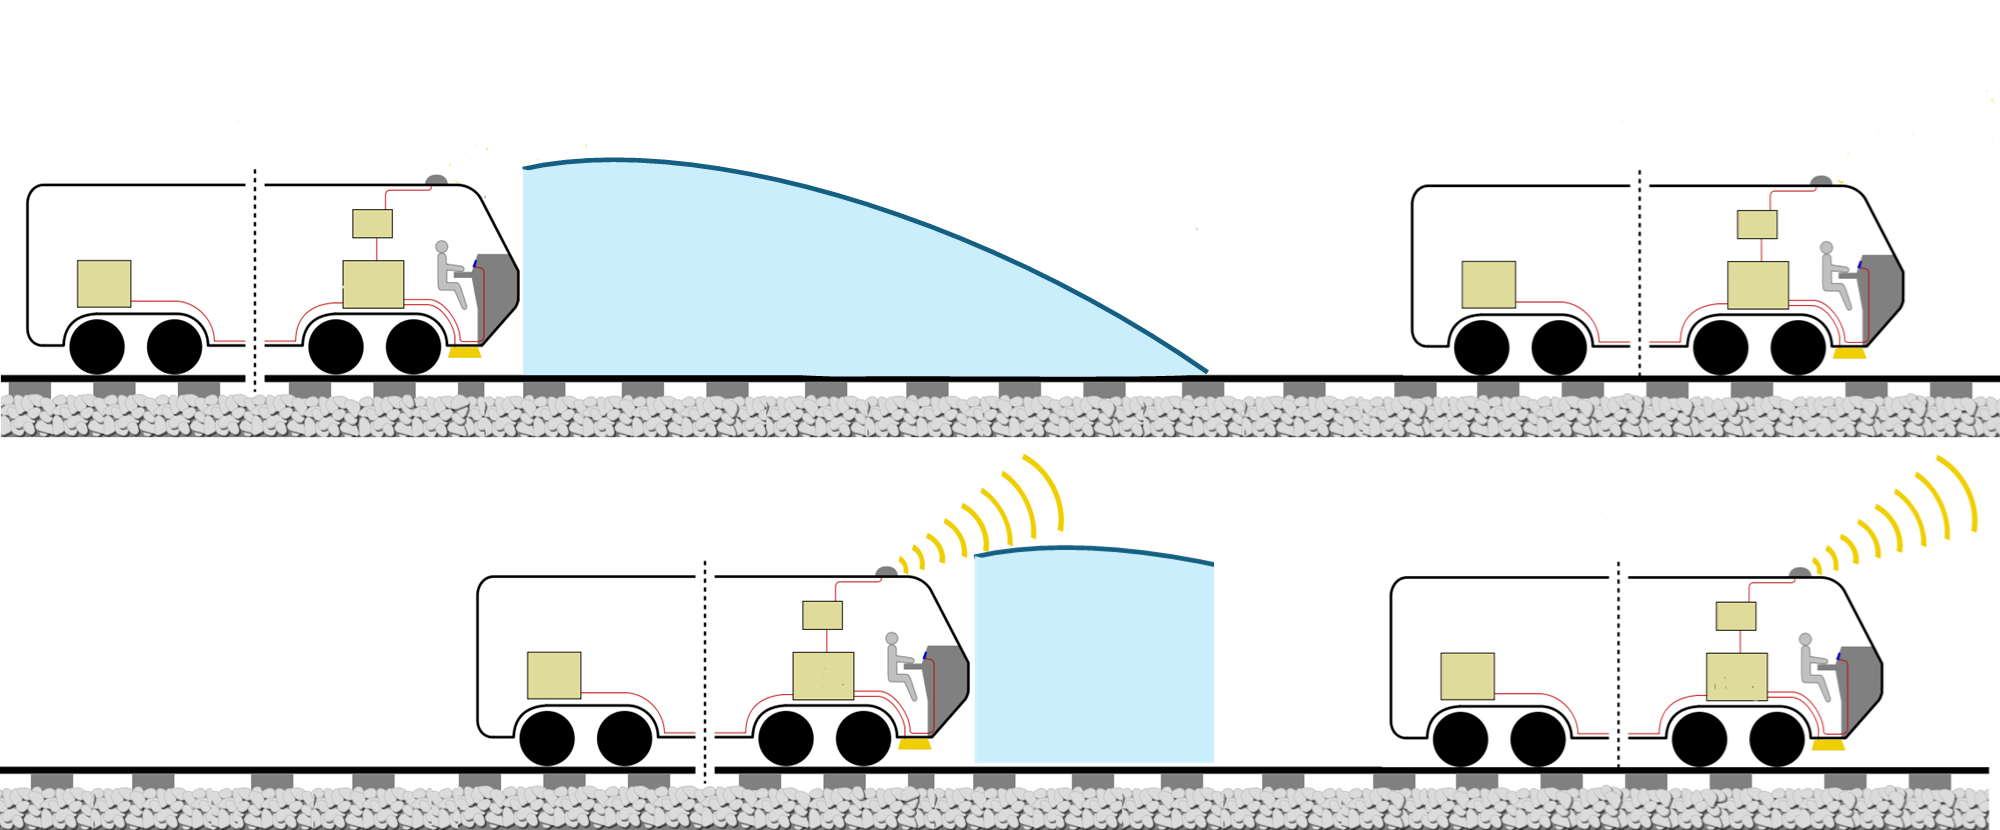
\includegraphics[width=623.25pt,height=272.36pt]{figure/Part3/levels.png}};



% Text Node
\draw (-6.27,5.95) node   [draw, fill= lightgray, line width=0.75 mm, align=left] 
{\Huge {\fontfamily{ptm}\selectfont L3}};

% Text Node
\draw (-4.67,196.95) node   [draw, fill = lightgray, line width=0.75 mm, align=left] 
{\Huge {\fontfamily{ptm}\selectfont VC}};





,\end{tikzpicture}
}
	\caption{Comparison scenarios between \gls{l3} and \gls{vc}.
		The blue area beneath the curve represents the absolute braking distance required to stop the train.}
	\label{fig:ertmsl3vc}
\end{figure}

In conclusion, \gls{vc} presents a notable advantage in reducing railway delays, particularly in departure times. This innovative system holds the potential to decrease departure delays by optimizing train coordination and spacing. Promoting a more synchronized and efficient operation, virtual coupling emerges as a valuable solution to increase the capacity and the enhance punctuality across the railway network.
%
\subsection{Related Works}
\label{subsec:relatedWorks}

A fair amount of work exists on the topic of \gls{vc} and in particular regarding the control techniques developed~\cite{wu2023railway}. The main technologies mentioned include: consensus-based control~\cite{wu2023dynamics}, constraint following control~\cite{zhang2023optimal,wang2022constraint}, sliding mode control~\cite{park2022,liu2023method}, \gls{mpc}, and \gls{ml}-based control. Emphasis will be given to the last two types, as they prove to be the most promising in this field; specifically, the latter is the type upon which the control system presented in this paper is based.

The integration of \gls{ml} into control algorithms has gained significant attention in the context of railway systems, particularly concerning virtual coupling~\cite{basile2022roadmap}. In~\cite{wang2021}, the use of \gls{rl} is proposed to obtain an optimal policy for IoT-based \gls{vcts}. The proposed approach combines \gls{rl} and artificial potential field to achieve global optimal policy and increase efficiency. Simulation results demonstrate the effectiveness of the proposed \gls{rl}-based cooperative control approach for IoT-based \gls{vcts}. And \cite{basile2022}, a \gls{ddpg} controller is proposed for \gls{vc} control in uncertain autonomous trains convoys. The proposed controller tracks the reference behavior imposed by the \gls{rbc} and maintains the desired inter-train distance with respect to the preceding train. 
%
The bottleneck of this innovative \gls{ml}-based control type lies in the foundations of its theory. Currently, in the railway domain, it is not yet possible to certify an \gls{ml}-based controller according to railway safety standards.

The approaches most closely related to our solution are the works in~\cite{felez2019model} and~\cite{wu2021virtually}. In~\cite{felez2019model} is introduced a novel train control system using virtual coupling. It employs a decentralized model predictive control framework for convoy trains, optimizing control for both leading and following trains. Comparative analyses, particularly against the moving block system, reveal improved performance, demonstrating the virtual coupling's efficacy in reducing headway and ensuring safe train separation. A linear \gls{mpc} optimizing goals like track spacing, velocity, and comfort is implemented in ~\cite{wu2021virtually}. Constraints, including line speed, collision avoidance, and traction/braking, are considered. In this work, although they utilize safety constraints inside the controller no certification of safety is demonstrated. Moreover, compared with these two contributions, our control scheme takes into account the intrinsic characteristics of the communication channel and assumes a heterogeneous platoon with parameters uncertainty. In both, the authors propose a decentralized linear \glspl{mpc} to realize the \gls{vc}; in this design control choice  lies another important distinction compared to our implementation employing a \gls{h-nmpc}. In conclusion, the two proposed solution implement \gls{mpc} controllers which have computation times that render them unsuitable for real-time usage; in contrast, our work use a millisecond Hybrid-\gls{nmpc} which places the use of \glspl{mpc}-based control algorithms as a viable solution for the \gls{vc}.
%
\subsection{Contribution}
\label{subsec:contribution}
%

In this article, we introduce a control system architecture that addresses the transition from \gls{l3} to \gls{vc} and manage \gls{vc} operation. 

The significance and original contributions of our work are articulated through the following key points:

\begin{enumerate}
	
	\item Our problem formulation addresses the dual challenges of parameter uncertainty within train system models and the variability in communication channel characteristics. We establish a robust control system framework that is specifically engineered to accommodate these variabilities, ensuring reliable performance across a broad spectrum of operational conditions.
	
	
	\item We incorporate a safety-critical barrier function into the design of our control system. This integration, supported by an \gls{ecd} mechanism derived from the barrier function, guarantees the safety of the system, affirming our commitment to prioritizing operational security.
	
	\item The control system implements an \gls{h-nmpc}, which integrates the aforementioned barrier function into its formulation. The adoption of the Proximal Averaged Newton-type method for Optimal Control significantly enhances computational efficiency, achieving processing speeds in the millisecond range. This breakthrough underscores the system's suitability for real-time applications, showcasing its potential to significantly improve responsiveness and reliability.
	
	\item To validate the applicability and safety of our control system, we have developed a specialized railway simulation tool for \gls{vc} scenarios. This tool enables testing and evaluation of the control system across various scenarios. The demonstration of the system's effectiveness in these tests not only proves its operational viability but also solidifies its foundational role in advancing railway safety.
\end{enumerate}
%
The remainder of this paper is organized as follows: 
in Section \ref{sec:Background} introduces mathematical tools like the Barrier Function for safety certification and Channel Communication \gls{v2v} formulation . Section \ref{sec:TrainModeling} reports the longitudinal train model, addressing parametric uncertainties through robust modeling. Section \ref{sec:SafetyGuarantee} elaborates on mathematical models and definitions to support the safety guarantee; moreover, it reports a Safety Certificate Theorem ensuring that the system's design will maintain safety distances under all conditions, supported by mathematical proofs provided in an appendix.. The control system architecture, illustrated in Section \ref{sec:controlsystem}, transitioning from \gls{l3} to \gls{vc} with an novel \gls{h-nmpc} approach, is thoroughly explained. In the conclusive Section \ref{sec:conclusion} simulation results validate the system's effectiveness, followed by conclusions on its implications for railway safety and efficiency.








%%% END SECTION ============================================================
%%% START SECTION ==========================================================
\section{Background}
\label{sec:Background}


In this section, we provide a concise introduction to all the mathematical tools utilized within the paper. 



\subsection{Barrier Function}
\label{subsec:barrier}

In this study, we explore scenarios where the state of a dynamical system, represented by \(x \in \mathbb{R}^n\), is defined by the differential equation:
\begin{equation*}
	\dot{x} = f(x) + g(x)u,
\end{equation*}
where \(f: \mathbb{R}^n \to \mathbb{R}^n\) demonstrates local Lipschitz continuity, a condition necessary to guarantee the existence and uniqueness of the system's solutions. Our aim is to ensure that the system's state consistently conforms to a safety certificate \cite{belta}:
\begin{equation*}
	B(x) \leq 0,
\end{equation*}
with \(B: \mathbb{R}^n \to \mathbb{R}\) being a continuously differentiable function. According to Nagumo's theorem, the initial safety of the system, i.e., \(B(x(0)) \leq 0\), implies its ongoing safety, i.e., \(B(x(t)) \leq 0, \forall t \geq 0\), provided that
\begin{equation}
	\dot{B}(x) \leq 0 \text{, whenever } B(x) = 0.
\end{equation}

Here, \(B(x)\) acts as a barrier function for the system, ensuring that the state \(x\) is restricted to the boundary of the safe set, defined as \(\{x \in \mathbb{R}^n : B(x) \leq 0\}\). This principle is pivotal for the safety verification process and serves as a cornerstone for the safety certification of dynamical systems.

In this context, we define the safe set \(S\) as
\[ S := \left\{ x \in \mathbb{R}^n : B(x) \leq 0 \right\}. \]
A Control Barrier Function, relative to \(S\), is given by \(B(x)\) and requires a class \(\mathcal{K}\) function \(\epsilon\) to ensure that for all \(x\) in \(S\),
\begin{equation}
	\sup_{{u} \in U} \left[ L_f B(x) + L_g B(x) u + \epsilon(B(x)) \right] \leq 0, 
\end{equation}
where \(L_f\) and \(L_g\) represent the Lie derivatives relative to the system dynamics \(f\) and control inputs \(g\), respectively, with the condition that \(L_g B(x) \neq 0\) when \(B(x) = 0\).




\begin{comment}
	
	\section{Railway Infrastructure}
	\label{sec:RailwayInfrastructure}
	
	The proposed concept is adopted for the control system architecture depicted in \ref{fig:architecture}.
	%
	\begin{figure}[ht] \label{fig:architecture}
		\resizebox{\linewidth}{!}{


\tikzset{every picture/.style={line width=0.75pt}} %set default line width to 0.75pt        

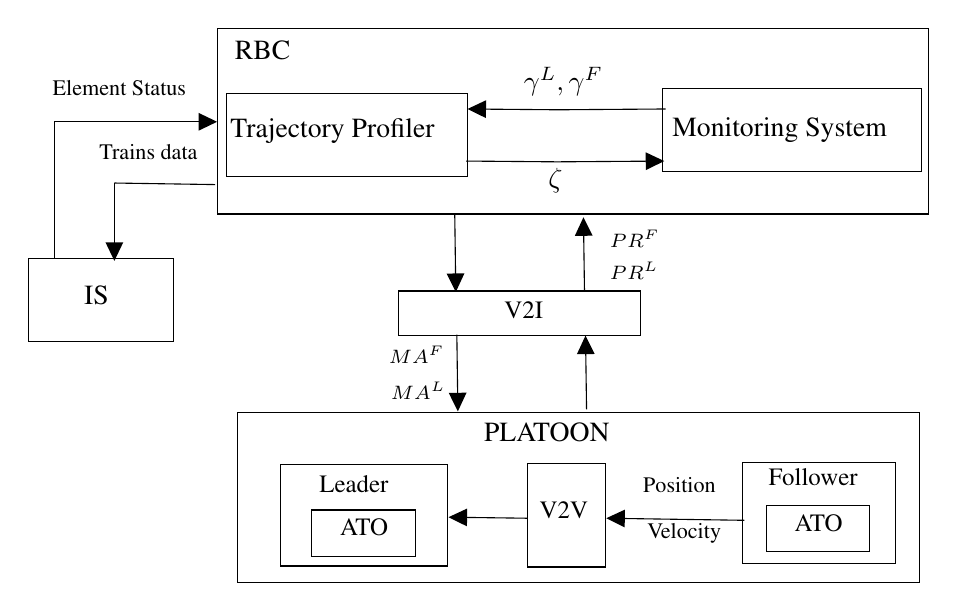
\begin{tikzpicture}[x=0.75pt,y=0.75pt,yscale=-1,xscale=1]
%uncomment if require: \path (0,300); %set diagram left start at 0, and has height of 300

%Shape: Rectangle [id:dp9181587437923022] 
\draw   (172,122.67) -- (242,122.67) -- (242,162.67) -- (172,162.67) -- cycle ;
%Shape: Rectangle [id:dp20903442434187935] 
\draw   (263,11.67) -- (605.67,11.67) -- (605.67,101.17) -- (263,101.17) -- cycle ;
%Shape: Rectangle [id:dp41239476881753845] 
\draw   (273,197) -- (601.5,197) -- (601.5,278.75) -- (273,278.75) -- cycle ;
%Shape: Rectangle [id:dp530653774898959] 
\draw   (267.67,43) -- (383.67,43) -- (383.67,83) -- (267.67,83) -- cycle ;
%Shape: Rectangle [id:dp07362802641529798] 
\draw   (477.56,40.83) -- (602.33,40.83) -- (602.33,80.83) -- (477.56,80.83) -- cycle ;
%Shape: Rectangle [id:dp3493633693136575] 
\draw   (293.5,221.83) -- (374,221.83) -- (374,270.75) -- (293.5,270.75) -- cycle ;
%Shape: Rectangle [id:dp34089559436294614] 
\draw   (350.5,138.25) -- (466.83,138.25) -- (466.83,159.5) -- (350.5,159.5) -- cycle ;
%Shape: Rectangle [id:dp38792726766554986] 
\draw   (412.5,221.25) -- (450,221.25) -- (450,271.25) -- (412.5,271.25) -- cycle ;
%Straight Lines [id:da41264737503221705] 
\draw    (383,75.67) -- (426.84,76.04) -- (475.44,75.69) ;
\draw [shift={(478.44,75.67)}, rotate = 179.58] [fill={rgb, 255:red, 0; green, 0; blue, 0 }  ][line width=0.08]  [draw opacity=0] (8.93,-4.29) -- (0,0) -- (8.93,4.29) -- cycle    ;
%Straight Lines [id:da35026960584329925] 
\draw    (377.5,101.75) -- (377.96,135.75) ;
\draw [shift={(378,138.75)}, rotate = 269.23] [fill={rgb, 255:red, 0; green, 0; blue, 0 }  ][line width=0.08]  [draw opacity=0] (8.93,-4.29) -- (0,0) -- (8.93,4.29) -- cycle    ;
%Straight Lines [id:da16469888193523596] 
\draw    (378.5,159.25) -- (378.96,193.25) ;
\draw [shift={(379,196.25)}, rotate = 269.23] [fill={rgb, 255:red, 0; green, 0; blue, 0 }  ][line width=0.08]  [draw opacity=0] (8.93,-4.29) -- (0,0) -- (8.93,4.29) -- cycle    ;
%Straight Lines [id:da8472970357726008] 
\draw    (440,138.25) -- (439.54,105.75) ;
\draw [shift={(439.5,102.75)}, rotate = 89.19] [fill={rgb, 255:red, 0; green, 0; blue, 0 }  ][line width=0.08]  [draw opacity=0] (8.93,-4.29) -- (0,0) -- (8.93,4.29) -- cycle    ;
%Straight Lines [id:da2638037577347745] 
\draw    (441,195.25) -- (440.54,162.75) ;
\draw [shift={(440.5,159.75)}, rotate = 89.19] [fill={rgb, 255:red, 0; green, 0; blue, 0 }  ][line width=0.08]  [draw opacity=0] (8.93,-4.29) -- (0,0) -- (8.93,4.29) -- cycle    ;
%Shape: Rectangle [id:dp711774726571057] 
\draw   (516.33,220.83) -- (590,220.83) -- (590,269.75) -- (516.33,269.75) -- cycle ;
%Shape: Rectangle [id:dp3073038779813597] 
\draw   (308.5,243.79) -- (358.5,243.79) -- (358.5,266) -- (308.5,266) -- cycle ;
%Shape: Rectangle [id:dp744059415491537] 
\draw   (527.5,241.46) -- (577.5,241.46) -- (577.5,263.67) -- (527.5,263.67) -- cycle ;
%Straight Lines [id:da7367089023216331] 
\draw    (184.5,56.75) -- (260,56.75) ;
\draw [shift={(263,56.75)}, rotate = 180] [fill={rgb, 255:red, 0; green, 0; blue, 0 }  ][line width=0.08]  [draw opacity=0] (8.93,-4.29) -- (0,0) -- (8.93,4.29) -- cycle    ;
%Straight Lines [id:da5062815061117323] 
\draw    (184.5,56.75) -- (184.5,122.75) ;
%Straight Lines [id:da32086022579187445] 
\draw    (213.5,86.25) -- (213.5,120.75) ;
\draw [shift={(213.5,123.75)}, rotate = 270] [fill={rgb, 255:red, 0; green, 0; blue, 0 }  ][line width=0.08]  [draw opacity=0] (8.93,-4.29) -- (0,0) -- (8.93,4.29) -- cycle    ;
%Straight Lines [id:da9349544027263015] 
\draw    (262,87) -- (213.5,86.25) ;
%Straight Lines [id:da8061807028246681] 
\draw    (517,248.75) -- (453.5,247.8) ;
\draw [shift={(450.5,247.75)}, rotate = 0.86] [fill={rgb, 255:red, 0; green, 0; blue, 0 }  ][line width=0.08]  [draw opacity=0] (8.93,-4.29) -- (0,0) -- (8.93,4.29) -- cycle    ;
%Straight Lines [id:da25677830767358123] 
\draw    (412.5,247.75) -- (377.5,247.29) ;
\draw [shift={(374.5,247.25)}, rotate = 0.75] [fill={rgb, 255:red, 0; green, 0; blue, 0 }  ][line width=0.08]  [draw opacity=0] (8.93,-4.29) -- (0,0) -- (8.93,4.29) -- cycle    ;
%Straight Lines [id:da4316689504126945] 
\draw    (386.62,50.61) -- (427.45,50.96) -- (479.06,50.58) ;
\draw [shift={(383.62,50.58)}, rotate = 0.49] [fill={rgb, 255:red, 0; green, 0; blue, 0 }  ][line width=0.08]  [draw opacity=0] (8.93,-4.29) -- (0,0) -- (8.93,4.29) -- cycle    ;

% Text Node
\draw (197.67,134.33) node [anchor=north west][inner sep=0.75pt]   [align=left] {{\fontfamily{ptm}\selectfont IS}};
% Text Node
\draw (270.33,16.17) node [anchor=north west][inner sep=0.75pt]   [align=left] {{\fontfamily{ptm}\selectfont RBC}};
% Text Node
\draw (268.17,53.83) node [anchor=north west][inner sep=0.75pt]   [align=left] {{\fontfamily{ptm}\selectfont Trajectory Profiler}};
% Text Node
\draw (481.06,53.58) node [anchor=north west][inner sep=0.75pt]  [font=\normalsize] [align=left] {{\fontfamily{ptm}\selectfont Monitoring System}};
% Text Node
\draw (400.17,142) node [anchor=north west][inner sep=0.75pt]  [font=\small] [align=left] {{\fontfamily{ptm}\selectfont {\small V2I}}};
% Text Node
\draw (417.17,238.5) node [anchor=north west][inner sep=0.75pt]  [font=\small] [align=left] {{\fontfamily{ptm}\selectfont {\small V2V}}};
% Text Node
\draw (390.33,200.33) node [anchor=north west][inner sep=0.75pt]   [align=left] {{\fontfamily{ptm}\selectfont PLATOON}};
% Text Node
\draw (311,225.83) node [anchor=north west][inner sep=0.75pt]  [font=\small] [align=left] {{\fontfamily{ptm}\selectfont Leader}};
% Text Node
\draw (527.5,222.33) node [anchor=north west][inner sep=0.75pt]  [font=\small] [align=left] {{\fontfamily{ptm}\selectfont Follower}};
% Text Node
\draw (321,246.83) node [anchor=north west][inner sep=0.75pt]  [font=\small] [align=left] {{\small {\fontfamily{ptm}\selectfont ATO}}};
% Text Node
\draw (540,244.5) node [anchor=north west][inner sep=0.75pt]  [font=\small] [align=left] {{\small {\fontfamily{ptm}\selectfont ATO}}};
% Text Node
\draw (345.5,180.9) node [anchor=north west][inner sep=0.75pt]  [font=\scriptsize]  {$MA^{L}$};
% Text Node
\draw (344.5,163.4) node [anchor=north west][inner sep=0.75pt]  [font=\scriptsize]  {$MA^{F}$};
% Text Node
\draw (451,107.4) node [anchor=north west][inner sep=0.75pt]  [font=\scriptsize]  {$PR^{F}$};
% Text Node
\draw (451,122.9) node [anchor=north west][inner sep=0.75pt]  [font=\scriptsize]  {$PR^{L}$};
% Text Node
\draw (467,227) node [anchor=north west][inner sep=0.75pt]   [align=left] {{\fontfamily{ptm}\selectfont {\footnotesize Position}}};
% Text Node
\draw (469,249) node [anchor=north west][inner sep=0.75pt]   [align=left] {{\fontfamily{ptm}\selectfont {\footnotesize Velocity}}};
% Text Node
\draw (205,66.33) node [anchor=north west][inner sep=0.75pt]   [align=left] {{\fontfamily{ptm}\selectfont {\footnotesize Trains data}}};
% Text Node
\draw (182.5,35.5) node [anchor=north west][inner sep=0.75pt]  [font=\normalsize] [align=left] {{\footnotesize {\fontfamily{ptm}\selectfont Element Status}}};
% Text Node
\draw (421.33,77.73) node [anchor=north west][inner sep=0.75pt]    {$\zeta $};
% Text Node
\draw (409.58,29.26) node [anchor=north west][inner sep=0.75pt]    {$\gamma ^{L} ,\gamma ^{F}$};


\end{tikzpicture}

}
		\caption{Architecture proposed.}
		\label{fig:architecture}
	\end{figure}
	
	Here, the \gls{rbc} is the critical component of the railway infrastructure during the transition level, it is entrusted with the task of generating safe trajectories for the platoon components in such a way that at the end of the transition the latter are in the \gls{vc} state. The block MA Dispatcher is in charge to compute the safe margin $S_\mathrm{VC}$ and coupling velocity $V_\mathrm{VC}$. Once the Trajectory Profiler calculates the velocity trajectories using the information positions (i.e. \glspl{pr}) obtained from the trains, these are encapsulated in \gls{ertms} messages and are sent in the form of \glspl{ma} to the trains. When the \gls{vc} state is reached,  in this phase the infrastructure will only have the task of supervising and monitoring the information coming from the platoon.
	
	Two communication interface are present: \gls{v2i}, which allows the trains to exchange data information with the \gls{rbc}; and \gls{v2v}, which allows platoon components to transmit their data to each other. These two communication channels will be defined in the Subsection \ref{subsec:communication}.
	
	The platoon, which is composed of a Leader and a Follower train, is the core of the railway operation. During the Transition Level, both \glspl{ato}, that is the onboard train local controller, follows the velocity trajectories acquired by the Infrastructure. Along the paper the superscript $\mathrm{\mathrm{L}}$ and $\mathrm{\mathrm{F}}$ will refer to Leader and Follower, respectively.
	
	Instead, In \gls{vc} state the Leader takes the lead and sets the pace of the platoon, while the Follower follows the leader. Within this operation state, the controller inside the \gls{ato} present into the Follower, is designed to support \gls{vc} functionality. In particular, using the \gls{v2v} the leader transmits its data information. 
	%
	\subsection{Operational Process}
	\label{subsec:operationalProcess}
	%
	The entire process is structured as a state machine in \ref{fig:stateMachine}, encompassing four distinct states: \gls{l3},  \gls{l3}$\rightleftarrows$\gls{vc}, \gls{vc} and \textrm{EM}. 
	
	\begin{figure}[ht] \label{fig:stateMachine}
		\resizebox{\linewidth}{!}{


\tikzset{every picture/.style={line width=0.75pt}} %set default line width to 0.75pt        

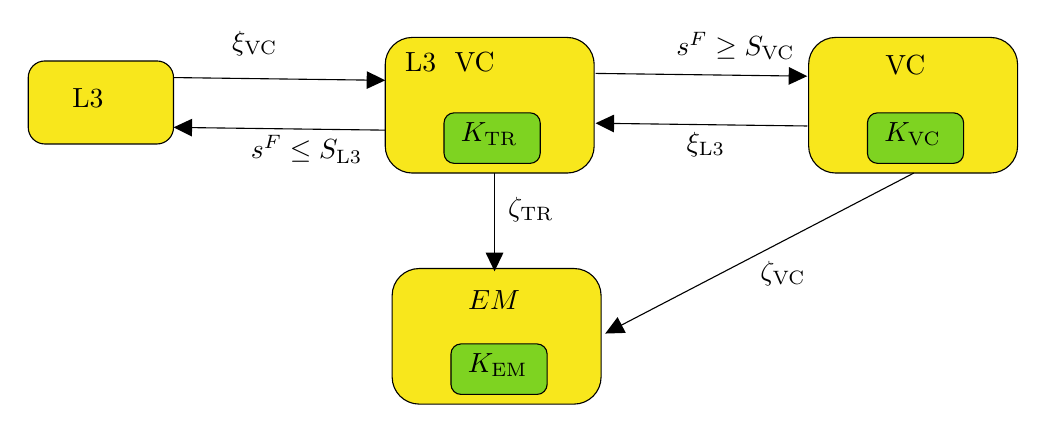
\begin{tikzpicture}[x=0.75pt,y=0.75pt,yscale=-1,xscale=1]
%uncomment if require: \path (0,300); %set diagram left start at 0, and has height of 300

%Rounded Rect [id:dp24689060389445716] 
\draw  [fill={rgb, 255:red, 248; green, 231; blue, 28 }  ,fill opacity=1 ] (105,135.67) .. controls (105,131.25) and (108.58,127.67) .. (113,127.67) -- (167,127.67) .. controls (171.42,127.67) and (175,131.25) .. (175,135.67) -- (175,159.67) .. controls (175,164.08) and (171.42,167.67) .. (167,167.67) -- (113,167.67) .. controls (108.58,167.67) and (105,164.08) .. (105,159.67) -- cycle ;
%Rounded Rect [id:dp03990125264398037] 
\draw  [fill={rgb, 255:red, 248; green, 231; blue, 28 }  ,fill opacity=1 ] (277,129.4) .. controls (277,122.18) and (282.85,116.33) .. (290.07,116.33) -- (364.6,116.33) .. controls (371.82,116.33) and (377.67,122.18) .. (377.67,129.4) -- (377.67,168.6) .. controls (377.67,175.82) and (371.82,181.67) .. (364.6,181.67) -- (290.07,181.67) .. controls (282.85,181.67) and (277,175.82) .. (277,168.6) -- cycle ;
%Rounded Rect [id:dp7956869543382266] 
\draw  [fill={rgb, 255:red, 126; green, 211; blue, 33 }  ,fill opacity=1 ] (305.33,157.53) .. controls (305.33,154.85) and (307.51,152.67) .. (310.2,152.67) -- (346.8,152.67) .. controls (349.49,152.67) and (351.67,154.85) .. (351.67,157.53) -- (351.67,172.13) .. controls (351.67,174.82) and (349.49,177) .. (346.8,177) -- (310.2,177) .. controls (307.51,177) and (305.33,174.82) .. (305.33,172.13) -- cycle ;

%Rounded Rect [id:dp9718527933811503] 
\draw  [fill={rgb, 255:red, 248; green, 231; blue, 28 }  ,fill opacity=1 ] (481,129.4) .. controls (481,122.18) and (486.85,116.33) .. (494.07,116.33) -- (568.6,116.33) .. controls (575.82,116.33) and (581.67,122.18) .. (581.67,129.4) -- (581.67,168.6) .. controls (581.67,175.82) and (575.82,181.67) .. (568.6,181.67) -- (494.07,181.67) .. controls (486.85,181.67) and (481,175.82) .. (481,168.6) -- cycle ;
%Rounded Rect [id:dp4375862505854522] 
\draw  [fill={rgb, 255:red, 126; green, 211; blue, 33 }  ,fill opacity=1 ] (509.33,157.53) .. controls (509.33,154.85) and (511.51,152.67) .. (514.2,152.67) -- (550.8,152.67) .. controls (553.49,152.67) and (555.67,154.85) .. (555.67,157.53) -- (555.67,172.13) .. controls (555.67,174.82) and (553.49,177) .. (550.8,177) -- (514.2,177) .. controls (511.51,177) and (509.33,174.82) .. (509.33,172.13) -- cycle ;

%Rounded Rect [id:dp876279933975634] 
\draw  [fill={rgb, 255:red, 248; green, 231; blue, 28 }  ,fill opacity=1 ] (280.33,240.73) .. controls (280.33,233.52) and (286.18,227.67) .. (293.4,227.67) -- (367.93,227.67) .. controls (375.15,227.67) and (381,233.52) .. (381,240.73) -- (381,279.93) .. controls (381,287.15) and (375.15,293) .. (367.93,293) -- (293.4,293) .. controls (286.18,293) and (280.33,287.15) .. (280.33,279.93) -- cycle ;
%Rounded Rect [id:dp039461928783934175] 
\draw  [fill={rgb, 255:red, 126; green, 211; blue, 33 }  ,fill opacity=1 ] (308.67,268.87) .. controls (308.67,266.18) and (310.85,264) .. (313.53,264) -- (350.13,264) .. controls (352.82,264) and (355,266.18) .. (355,268.87) -- (355,283.47) .. controls (355,286.15) and (352.82,288.33) .. (350.13,288.33) -- (313.53,288.33) .. controls (310.85,288.33) and (308.67,286.15) .. (308.67,283.47) -- cycle ;

%Straight Lines [id:da8518584621470304] 
\draw    (175,135.67) -- (274,136.96) ;
\draw [shift={(277,137)}, rotate = 180.75] [fill={rgb, 255:red, 0; green, 0; blue, 0 }  ][line width=0.08]  [draw opacity=0] (8.93,-4.29) -- (0,0) -- (8.93,4.29) -- cycle    ;
%Straight Lines [id:da31078013867281284] 
\draw    (178,159.71) -- (277,161) ;
\draw [shift={(175,159.67)}, rotate = 0.75] [fill={rgb, 255:red, 0; green, 0; blue, 0 }  ][line width=0.08]  [draw opacity=0] (8.93,-4.29) -- (0,0) -- (8.93,4.29) -- cycle    ;
%Straight Lines [id:da5622985546516415] 
\draw    (378.33,133.67) -- (477.33,134.96) ;
\draw [shift={(480.33,135)}, rotate = 180.75] [fill={rgb, 255:red, 0; green, 0; blue, 0 }  ][line width=0.08]  [draw opacity=0] (8.93,-4.29) -- (0,0) -- (8.93,4.29) -- cycle    ;
%Straight Lines [id:da8651290950592201] 
\draw    (381.33,157.71) -- (480.33,159) ;
\draw [shift={(378.33,157.67)}, rotate = 0.75] [fill={rgb, 255:red, 0; green, 0; blue, 0 }  ][line width=0.08]  [draw opacity=0] (8.93,-4.29) -- (0,0) -- (8.93,4.29) -- cycle    ;
%Straight Lines [id:da9169685244420764] 
\draw    (329.67,181.67) -- (329.67,226) ;
\draw [shift={(329.67,229)}, rotate = 270] [fill={rgb, 255:red, 0; green, 0; blue, 0 }  ][line width=0.08]  [draw opacity=0] (8.93,-4.29) -- (0,0) -- (8.93,4.29) -- cycle    ;
%Straight Lines [id:da5583832122874837] 
\draw    (531.67,181.67) -- (385.66,257.62) ;
\draw [shift={(383,259)}, rotate = 332.52] [fill={rgb, 255:red, 0; green, 0; blue, 0 }  ][line width=0.08]  [draw opacity=0] (8.93,-4.29) -- (0,0) -- (8.93,4.29) -- cycle    ;

% Text Node
\draw (125,139.73) node [anchor=north west][inner sep=0.75pt]    {$\mathrm{L3}$};
% Text Node
\draw (516.67,123.73) node [anchor=north west][inner sep=0.75pt]    {$\mathrm{VC}$};
% Text Node
\draw (516.2,156.07) node [anchor=north west][inner sep=0.75pt]    {$K_{\mathrm{VC}}$};
% Text Node
\draw (315.67,237.07) node [anchor=north west][inner sep=0.75pt]    {$EM$};
% Text Node
\draw (315.53,267.4) node [anchor=north west][inner sep=0.75pt]    {$K_{\mathrm{EM}}$};
% Text Node
\draw (312.2,156.07) node [anchor=north west][inner sep=0.75pt]    {$K_{\mathrm{TR}}$};
% Text Node
\draw (285.33,122.4) node [anchor=north west][inner sep=0.75pt]    {$\mathrm{L3}\ \rightleftarrows \ \mathrm{VC}$};
% Text Node
\draw (335,191.9) node [anchor=north west][inner sep=0.75pt]    {$\zeta _{\mathrm{TR}}$};
% Text Node
\draw (456.5,222.9) node [anchor=north west][inner sep=0.75pt]    {$\zeta _{\mathrm{VC}}$};
% Text Node
\draw (211,162.4) node [anchor=north west][inner sep=0.75pt]    {$s^F \leq S_{\mathrm{L3}}$};
% Text Node
\draw (416,112.4) node [anchor=north west][inner sep=0.75pt]    {$s^F \geq S_{\mathrm{VC}}$};
% Text Node
\draw (202,111.9) node [anchor=north west][inner sep=0.75pt]    {$\xi _{\mathrm{VC}}$};
% Text Node
\draw (421,160.9) node [anchor=north west][inner sep=0.75pt]    {$\xi _{\mathrm{L3} }$};


\end{tikzpicture}

}
		\caption{Control system state machine.}
	\end{figure}
	%
	For the sake of clarity, we initiate this process from the \gls{l3} state, where the Leader and Follower travel with a separation distance $S_{\mathrm{L3}}$. During this state, the two trains communicate their availability to perform a \gls{vc} to the \gls{rbc}; if the latter, considering the current state of the trains present on the infrastructure, agrees by setting true the acknowledgment $\xi _{\mathrm{VC} }$ to the trains. 
	
	After receiving the acknowledgment, the state machine enters in \gls{l3}$\rightleftarrows$\gls{vc}. This state has the goal to bring the trains from \gls{l3} to \gls{vc} and vice versa. In order for this to take place, the controller  $K_{\mathrm{TR}}$, as described in \ref{subsec:atoTransitionLevel},is utilized to track the trajectories that the \gls{rbc} has previously calculated and transmitted.
	
	Once the Follower's position reaches $S_{\mathrm{VC}}$, both trains find themselves in the \gls{vc} state. Throughout the entire duration of this state, the Follower will employ controller $K_{\mathrm{VC}}$, as detailed in  \red{\ref{subsec:atoTransitionLevel}}, while the Leader will continue to maintain control using the previously mentioned $K_{\mathrm{TR}}$. In the event of uncoupling requested by the \gls{rbc} through the $\xi _{\mathrm{L3} }$ request, the trains will revert to the previous \gls{l3}$\rightleftarrows$\gls{vc} state.
	
	The final EM state is activated in the event of an emergency during the stay in the two preceding states. Entry into this state is facilitated by the emergency flags $\zeta _{\mathrm{TR}}$ and $\zeta _{\mathrm{VC}}$. The controller $K_{\mathrm{EM}}$ selected for this state is described in \red{\ref{subsec:atoTransitionLevel}}.
	
	
	
	
	However, during the \textit{L3}$\rightarrow$\textit{VC} state, if the two trains establish a $\text{V2V}_{\text{\mathrm{L}}}$ communication, the state machine proceeds to the \textit{VC} state. Here, a robust switched \gls{nmpc} controllers $K_{\tau_1}, K_{\tau_2}$ and $K_{\tau_3}$, based on safety barrier functions detailed in section \ref{subsec:robustMPC}, are employed to manage this operational state. In the event of an emergency detected by the trains themselves, $\text{PLA}_{\text{C}}$ which will be defined in Section \ref{subsec:EventCollisionDetector}, or $\text{V2V}_{\text{\mathrm{L}}}$ communication is lost, or \gls{rbc} stops the virtual coupling operation state, in all these case the follower train equipped with an emergency controller $K_E$, will be utilized to transition the trains back to the \textit{L3} state.
	
	During the \textit{L3}$\leftarrow$\textit{VC} state, the controller steers the follower's position to a $S_{L3}$ distance relative to the leader. Upon reaching this point, both trains will revert to the \textit{L3} operational state. This process is pivotal in ensuring a smooth and safe transition from the virtual coupling mode to the standard Level 3 operation, maintaining a secure separation distance between the two trains as required by the existing protocol.
	
	The entire process is structured as a state machine wich have $4$ state: \gls{l3}, \gls{l3vc}, \gls{l3vc} and \gls{vcl3}. For the sake of simplicity we suppose to start from state \gls{l3}, here the two trains are travelling with a distance $d_{L3}$ and communicate to the infrastructure their availability to perform a \gls{vc}. Is an \gls{rbc} decision to create a \gls{vc}, this is obvious because only the infrastructure has a highest point of view on the railway traffic respect to the trains. Once that the \gls{rbc} decide for a \gls{vc} operation and computed the corresponding trajectories for the trains and sent by \gls{ma} the state arrive in \gls{l3vc}.
\end{comment}
%
\subsection{Channel Communication}
\label{subsec:transmissionEvent}
%
%
In this study, we examine the dynamics of train communication within systems operating under the European Train Control System (\gls{ertms}), which traditionally utilize an Event-Triggered transmission protocol. This approach entails the transmission of signals or messages in response to specific operational events or conditions. We specifically consider the challenges posed by communication delays and packet loss within the \gls{v2v} context.

In particular, the end-to-end delay $\tau$ is the total time delay between trains during \gls{v2v}. This delay is influenced by various factors, e.g. stochastic properties of channel communication and hardware processing time; furthermore, $\tau$  is  critical for the control system design under examination. To this end, it has been treated as a random variable, considering its stochastic nature is  approximated with the following exponential probability distribution 
%
\begin{equation} \label{eq:pdfDelay}
	\tau \sim F_{\mathrm{d}} (t;\lambda) = \begin{cases}\lambda e^{-\lambda (t-T_\mathrm{min})} & t \geq T_\mathrm{min}, \\ 0 & \text{otherwise},\end{cases}
\end{equation}
where $T_\mathrm{min}$ is the minimum time and $\lambda$ is the distribution's parameter.


Regarding the probabilistic characterization of packet loss, it is assumed to follow a Bernoulli distribution
\begin{equation} \label{pr_packet_loss}
	F_{\mathrm{pl}}(X = k) = \binom{n}{k} q^k  (1-q)^{n-k},
\end{equation}
where $q$  is the probability of not receiving the packet, $n$ is the total number of packets sent, $k$ is the number of packet losses, and $\binom{n}{k}$ represents the binomial coefficient, which calculates the number of packet losses that can occur out of $n$ packets sent.

Although this distribution is, in reality, dependent on multiple variables such as distances and velocities between the two communication systems and effects due to the environment, a simpler distribution is employed.

The Leader transmits its information, from the current value up to a horizon \(H\), at a period of \(T_{\text{comm}}\) at predefined synchronous moments, denoted as \(t_{\kappa^\mathrm{L}}\), with the sequence being \(\{ t_{\kappa^\mathrm{L}} \}_{\kappa^\mathrm{L}=0}^{+\infty}\). The Follower receives these data packets at moments \(t_{\kappa^{LF}}\), with its sequence as \(\{ t_{\kappa^\mathrm{LF}} \}_{\kappa^\mathrm{LF}=0}^{+\infty}\).
%
In the following discussion two cases will be used for the sake of simplicity:
%
\begin{enumerate}
	\item \label{enum:channel1} The first scenario assumes no delays or packet drops, aligning the sequences of the Leader and Follower: 
	\[\{ t_{\kappa^\mathrm{L}} \}_{\kappa^\mathrm{L}=0}^{+\infty} = \{ t_{\kappa^\mathrm{LF}} \}_{\kappa^\mathrm{LF}=0}^{+\infty}.\]
	
	\item \label{enum:channel2} The second scenario accounts for the presence of delays and packet drops, resulting in the Follower receiving data packets at asynchronous moments or potentially not receiving them at all, thus: 
	\[\{ t_{\kappa^\mathrm{L}} \}_{\kappa^\mathrm{L}=0}^{+\infty} \neq \{ t_{\kappa^\mathrm{LF}} \}_{\kappa^\mathrm{LF}=0}^{+\infty}.\]
\end{enumerate}

Additionally, the following functions are defined to represent the last trigger times for the Leader and Follower, respectively, enabling a precise analysis of data transmission timing
\begin{align*}
	\ell_{\kappa^\mathrm{L}}(t) &= \max_{t_{\kappa^\mathrm{L}} \leq t} \left \{ t_{\kappa^\mathrm{L}} \right \}_{\kappa^\mathrm{L}=0}^{+\infty}, \\
	\ell_{\kappa^\mathrm{LF}}(t) &= \max_{t_{\kappa^\mathrm{LF}} \leq t} \left \{ t_{\kappa^\mathrm{LF}} \right \}_{\kappa^\mathrm{LF}=0}^{+\infty}.
\end{align*}
%


\section{Train Modeling}
\label{sec:TrainModeling}

The model employed in this manuscript relies on the principles of longitudinal train dynamics. It treats the train as a singular point mass with one degree of freedom. Additionally, it incorporates aspects such as the propulsion and braking system, the effects of rolling and bearing resistances, air input, the influence of aerodynamic drag, as well as the consideration of grade and curving resistances~\cite{ltdModel}:
%
\begin{align}  \label{eq:stateDynamic}
	\dot{x}_1^i &= x_2^i  \nonumber \\
	\dot{x}_2^i &= \frac{1}{M^i}(-A^i-B^i x_2^i - T_\mathrm{F}^i C^i (x_2^i)^2)-\mathrm{F}_e^i + \frac{u^i}{M^i}.
\end{align}
%

We utilize the symbols ${x}_1^i$ and ${x}_2^i$ to represent the $i$-th train's velocity $v^i$ and position $s^i$, respectively; the state vector is reported with $x^i=\binom{x^i_1}{x^i_2}$  along the present work. The variable $u^i$ is the control driving or braking force; $\mathrm{F}_e^i$ denotes the external force originating from the track; $M^i$ denotes the mass parameter, while $A^i$ encompasses both rolling resistance and bearing resistance; $B^i$ is a coefficient related to the flange friction, and $C^i$ represents the aerodynamic coefficient. Additionally, $T_\mathrm{F}$ denotes the tunnel factor.
%
In this model, $\mathrm{F}^i_e$ depends on $i$-th external force
%
\begin{equation*}
	\mathrm{F}_e^i = g \sigma(x_1^i) + \frac{\gamma}{\rho(x_1^i)}, 
\end{equation*}
%
where $\gamma=6\cdot10^6$ is a constant parameter. It encompasses two distinct constituents. The first term denotes the component attributed to gravity force resulting from the track's slope $\sigma(x_1^i)$  at point $x_1^i$, with $g$ representing the gravitational acceleration. The second term designates the curving resistance, with ${\rho(x_1^i)}$ representing the curve's radius.

Regarding the constraints on the state and input of the model, they are presented as follows
%
\begin{subequations} \label{eq:modelConstraints}
	\begin{align}
		u^i &\in \left[M^i a_{\mathrm{br}}^i, \;M^i a_{\mathrm{dr}}^i \right], \label{eq:lim1} \\
		u^i \cdot x_2^i&\in \left[P^i_{\mathrm{br}}, \;P^i_{\mathrm{dr}}\right], \label{eq:lim2} \\
		x_2^i &\in \left[0, \;\min\{V^i_{\mathrm{max}},V_{\mathrm{line}}\}\right], \label{eq:lim5} \\
		x_1^i &\in \mathbb{R}_{\geq0}, \label{eq:lim4}  \\ 
		\frac{\dot{u}^i }{M^i}&\in \left[-J^i_{\mathrm{max}}, \;J^i_{\mathrm{max}}\right]. \label{eq:lim3}
	\end{align}
\end{subequations}
%
Specifically, all of these parameters mentioned are contingent upon the constructional characteristics unique to each individual train. It is important to note that $a_{\mathrm{br}}^i \leq 0$ and $a_{\mathrm{dr}}^i \geq 0$ correspond to the maximum braking and acceleration admitted, $P^i_{\mathrm{br}}$ and $P^i_{\mathrm{dr}}$ represent the minimum and maximum mechanical power, $J^i_{\min}$ and $J^i_{\max}$  input rate of change, and finally, $V^i_{\max}$ and $V_{\mathrm{line}}$ denotes the maximum attainable velocity for the train and railway line, respectively.

\subsection{Robust Modeling}
\label{subsec:robustModeling}
%
In the context of railway control, and in particular, in this new technology the safety is of utmost importance, the integration of system model~\eqref{eq:stateDynamic} with parametric uncertainties is an essential step. 

For this purpose, the following model parameters are supposed uncertain in a given range
%
\begin{subequations}
	\begin{align*}
		&a_{\mathrm{br}}^i \in [\underline{a}_{\mathrm{br}}^i , \overline{a}_{\mathrm{br}}^i], \;
		a_{\mathrm{dr}}^i \in [\underline{a}_{\mathrm{dr}}^i , \overline{a}_{\mathrm{dr}}^i],  \;
		P^i_{\mathrm{br}} \in [\underline{P}_{\mathrm{br}}^i , \overline{P}_{\mathrm{br}}^i]  , \\
		&P^i_{\mathrm{dr}} \in [\underline{P}_{\mathrm{dr}}^i , \overline{P}_{\mathrm{dr}}^i],   \;
		T_\mathrm{F}^i \in [\underline{T}_\mathrm{F}^i , \overline{T}_\mathrm{F}^i] ,  \;
		J_\mathrm{max}^i \in [\underline{J}_\mathrm{max}^i , \overline{J}_\mathrm{max}^i] , \\
		&M^i \in [\underline{M}^i , \overline{M}^i], \;
		A^i \in [\underline{A}^i , \overline{A}^i] ,  \;
		B^i \in [\underline{B}^i , \overline{B}^i] , \;
		C^i \in [\underline{C}^i , \overline{C}^i].
	\end{align*}
\end{subequations}
%
The train model explicitly pointing out its dependency on the parameters listed above, appears as follows
%
\begin{equation}   \label{eq:robustModel}  
	\begin{cases}
		\dot{x}^i = f^i(x^i,u^i,p^i),  \\ 
		\text{subject to} \; \eqref{eq:modelConstraints} ,
	\end{cases}
\end{equation}
where $p^i \in P^i$, and
\begin{equation*}
	P^i = \{a_{\mathrm{br}}^i,\;  a_{\mathrm{dr}}^i,\;P^i_{\mathrm{br}},\;P^i_{\mathrm{dr}},\;T_\mathrm{F}^i,\;  J_\mathrm{max}^i,\;a_{\mathrm{dr}}^i,\;M^i,\;A^i ,\; B^i, \; C^i \}.
\end{equation*}
%
\begin{definition}[Braking Controller] \label{def:brakingController}
	Given the model present in \eqref{eq:robustModel} we define  $u^i= K_\mathrm{B}(x^i)$ the braking controller as follows
	\begin{equation*}
		K_B(x^i)=
		\begin{cases}
			\tilde{u}^i(x^i) \leq 0,& x_2^i \geq 0\\
			0 ,& x_2^i = 0.
		\end{cases}     
	\end{equation*}
\end{definition}
Defining $\phi^i(t,t_0,x_0^i,u^i,p^i)= \left [\begin{array}{c}
	\phi^i_1\left(\cdot \right) \\
	\phi^i_2\left(\cdot \right)
\end{array}\right ]$ as the dynamical flow for the parameterized model \eqref{eq:robustModel} and using the Definition reported in \ref{def:brakingController}, we introduce the following:
%
\begin{definition}[Stopping time] \label{def:stoppingTime}
	Given model present in \eqref{eq:robustModel}, we define the stopping time $t_{K_\mathrm{B}}$ for the braking controller  $u^i= K_\mathrm{B}(x^i)$ as
	\begin{equation*}
		t_{K_\mathrm{B}}: \underset{t \geq t_0}{\min}\{ t: \phi_2^i(t \;,t_0 \;,x_0^i, \;u^i(x^i), \;p^i)\}.
	\end{equation*}
\end{definition}
%
\subsection{Robust Proxies}
\label{subsec:robustProxies}
%
To address the dynamic nature of the system, considering a broad spectrum of parameters within fixed ranges, the notion of \gls{rlp} and \gls{rup} are introduced as robustification technique. By employing the latter, on the dynamical model~\eqref{eq:robustModel}, we aim to robustify the model's resilience against uncertainties, variations, and potential disturbances, ensuring across a diverse range of operating conditions. Ultimately, the utilization of robust and lower proxies has the goal of developing models that are robust and capable of accommodating the complexity and variability of real-world system.
%
\begin{definition}[\gls{rlp}]
	In consideration of the system expressed by Eq.~\eqref{eq:robustModel}, we formally introduce the \gls{rlp} as follows
	%
	\begin{equation} \label{eq:rlp}
		\underline{\dot{x}}^i = \underline{f}^i(\underline{x}^i,u^i).
	\end{equation}
\end{definition}

\begin{definition}[\gls{rup}]
	Similarly, we define the \gls{rup} for the model in~\eqref{eq:robustModel} as 
	\begin{equation} \label{eq:rup}
		\dot{\overline{x}}^i = \overline{f}^i(\overline{x}^i,u^i).
	\end{equation}
\end{definition}

As evident from the two definitions, there exist infinite proxy functions for Eq. \eqref{eq:robustModel}; in this work, we will consider piece-wise smooth discontinuous functions.

As for the \gls{rlp}, the following proxy has been chosen
\begin{equation}
	\begin{cases}
		\underline{\dot{x}}_1^i =   \underline{x}_2^i, \qquad  \qquad \qquad \qquad \qquad \qquad  \qquad  \text{if} \; u^i < 0,  \\
		\underline{\dot{x}}_2^i =  \frac{1}{\underline{M}^i} \left(-\overline{A}^i - \overline{B}^i \underline{x}^i_2 - \overline{T}^i_\mathrm{F} \overline{C}^i \left(\underline{x}^i_2\right)^2 \right)-\overline{F}_e^i + u^i, \\ \noalign{\vskip3pt}
		\textrm{with } \overline{F}_e^i =  g \sigma_{\sup}\left(\underline{x}^i_1\right)+ \frac{\gamma}{\rho_{\inf}\left(\underline{x}^i_1\right)} \\
		\noalign{\vskip9pt}
		\underline{\dot{x}}_1^i =   \underline{x}_2^i, \qquad \qquad \qquad  \qquad \qquad \qquad \qquad \text{if} \; u^i \geq 0,  \\
		\underline{\dot{x}}_2^i =  \frac{1}{\underline{M}^i} \left(-\overline{A}^i - \overline{B}^i \underline{x}^i_2 - \overline{T}^i_\mathrm{F} \overline{C}^i \left(\underline{x}^i_2\right)^2 \right)-\mathrm{F}_e^i  + u^i, \\
		\noalign{\vskip6pt}
		\textrm{subject to } \eqref{eq:modelConstraints} \textrm{, and where} \\
		\sigma_{\sup}\left(\underline{x}^i_1\right) = \underset{s \in [\underline{x}_1^i,s^H]}{\sup} \sigma(s), \\
		\rho_{\inf}\left(\underline{x}^i_1\right) = \underset{s \in [\underline{x}_1^i,s^H]}{\inf} \rho(s),
	\end{cases}
\end{equation}
here $s^H$ represent the position at the horizon control $H$.

Likewise to what was demonstrated above, we define here the proxy related to the \gls{rup}
\begin{equation}
	\begin{cases}
		\overline{\dot{x}}_1^i =   \overline{x}_2^i, \qquad  \qquad \qquad \qquad \qquad \qquad  \qquad  \text{if} \; u^i < 0,  \\
		\overline{\dot{x}}_2^i =  -\frac{\underline{A}^i}{\overline{M}^i}-\underline{F}_e^i + u^i, \\
		\textrm{with } \underline{F}_e^i =  g \sigma_{\inf}\left(\overline{x}^i_1\right)+ \frac{\gamma}{\rho_{sup}\left(\overline{x}^i_1\right)} \\
		\noalign{\vskip9pt}
		\overline{\dot{x}}_1^i =   \overline{x}_2^i, \qquad \qquad \qquad  \qquad \qquad \qquad \qquad \text{if} \; u^i \geq 0,  \\
		\overline{\dot{x}}_2^i =  \frac{1}{\overline{M}^i} \left(-\underline{A}^i - \underline{B}^i \overline{x}^i_2 - \underline{T}^i_\mathrm{F} \underline{C}^i \left(\overline{x}^i_2\right)^2 \right) -\mathrm{F}_e^i  + u^i, \\
		\noalign{\vskip5pt}
		\textrm{subject to } \eqref{eq:modelConstraints} \textrm{, and where} \\
		\sigma_{\sup}\left(\overline{x}^i_1\right) = \underset{s \in [\overline{x}_1^i,s^H]}{\inf} \sigma(s), \\
		\rho_{\inf}\left(\overline{x}^i_1\right) = \underset{s \in [\overline{x}_1^i,s^H]}{\sup} \rho(s).
	\end{cases}
\end{equation}

Hereinafter, we will use \gls{rlp} and \gls{rup} to refer to the two proxies, respectively.

\begin{lemma} \label{lemma:Proxies}
	Let ${\phi}^i(\cdot)$ the dynamical flow corresponding to \eqref{eq:robustModel}, $\underline{\phi}^i\left(\cdot \right)$ and   $\overline{\phi}^i\left(\cdot \right)$ represent the dynamical flow related to \eqref{eq:rlp} and \eqref{eq:rup}  then
	\begin{subequations}
		\begin{align} 
			&\underline{\phi}^i\left(t,t_0,x_0^i,u^i\right) \leq \phi^i\left(t,t_0,x_0^i,u^i,p^i\right), \label{lemma:rlpProxy}\\
			&\overline{\phi}^i\left(t,t_0,x_0^i,u^i\right) \geq \phi^i\left(t,t_0,x_0^i,u^i,p^i\right), \label{lemma:rupProxy}\\
			&\forall p^i \in P^i, \; \forall x_0^i \in X^i,\; \forall u^i \in U^i\left(x^i\right), \forall t \geq t_0, \nonumber
		\end{align}
	\end{subequations}
	where the inequalities are meant component-wise.
	\begin{proof}
		see Appendix \ref{appendix:proxy}.
	\end{proof}
\end{lemma}



\section{Safety Guarantee}
\label{sec:SafetyGuarantee}

The objective of the control system, introduced in \ref{sec:controlsystem}, is to ensure that the two trains maintain a safety separation distance. In other words, the goal is to guarantee that the distance between the Leader and Follower never falls below the predefined safety threshold $d$, that is
%
\begin{equation} \label{eq:distance}
	x_1^\mathrm{L}(t) - x_1^\mathrm{F}(t) \geq  \mathrm{L}^\mathrm{L} +d, \quad  \forall  t \in \mathbb{R}_{\geq 0},
\end{equation}
where $\mathrm{L}^\mathrm{L}$ is the Leader's length.

In order to satisfy the condition expressed in Eq.\tildeAdd\eqref{eq:distance} under any circumstances we will employ a Emergency Controller. It will enforce maximum braking on the Follower whenever there is a risk of collision with the Leader. 
%
\begin{definition}[Emergency Controller]
	We define  $u^i= K_\mathrm{E}(x^i)$ the emergency controller, for the model present in \eqref{eq:robustModel}, as follows
\end{definition}
\begin{equation*}
	K_E(x^i)=
	\begin{cases}
		\tilde{u}^i(x^i) =  \min\limits_{u^i \in U(x^i)} u^i(x), \;  &x_2^i \geq 0\\
		0 ,& x_2^i = 0
	\end{cases}       
\end{equation*}
%
The Emergency Controller activation is based on a suitable barrier function which will be introduced below.

From here until the end of the work, we consider the \gls{rlp} $\underline{f}^i(\underline{x}^{\mathrm{L}},K_B^\mathrm{L})$ for the Leader, where $K_B^\mathrm{L}$ is the Braking Controller with $\tilde{u}^\mathrm{L}\left(x^\mathrm{L}\right)= -\overline{a}^\mathrm{L}_\mathrm{br}$; and the \gls{rup} $\overline{f}^i(\overline{x}^{\mathrm{F}},K_B^\mathrm{F})$ for the Follower, where $K_B^\mathrm{F}\left(\overline{x}^\mathrm{F}\right)$ is with $\tilde{u}^\mathrm{F}\left(x^\mathrm{F}\right) = -\underline{\alpha}\left( t_0 \right)^\mathrm{F}$, where

\begin{equation*}
	\underline{\alpha}^i \left( t_0 \right)=\min \left\{-\underline{a}^i_\mathrm{br},\frac{\underline{P}_\mathrm{br}}{x_2^i}\left( t_0 \right) \right\}.
\end{equation*}


We compute the evolution of these two proxy values under the initial conditions of the Leader, denoted as $x^\mathrm{L}\left(t_0\right)=\left[s_0^\mathrm{L},v_0^\mathrm{L}\right]$, and the Follower, represented as $x^\mathrm{F}\left(t_0\right)=\left[s_0^\mathrm{F},v_0^\mathrm{F}\right]$. Calling
%
\begin{equation*}
	\begin{aligned}
		-\underline{e}^i\left(t_0\right)=\frac{1}{\underline{M}^i} & \left(-\overline{A}^i-\overline{B}^i x_2^i\left(t_0\right)-\overline{T}_\mathrm{F}^i \overline{C}^{i}\left(x_2^i\left(t_0\right)\right)^2\right)+ \\
		& -\left( g \sigma_{\sup}\left(t_0\right)+ \frac{\gamma}{\rho_{\inf}\left(t_0\right)} \right)-\overline{a}^i_\mathrm{br},
	\end{aligned}
\end{equation*}
%
we have that the \gls{rlp} stops at time
%
\begin{equation*}
	t_{K_B^\mathrm{L}} = \frac{v_0^\mathrm{L}}{\underline{e}^\mathrm{L}\left(t_0\right)} + t_0,
\end{equation*}
%
at position
%
\begin{equation*}
	\begin{aligned}
		\underline{x}_1^\mathrm{L}\left(t_{k_B^\mathrm{L}}\right) & =s_0^2+v_0^\mathrm{L} \frac{v_0^\mathrm{L}}{\underline{e}^\mathrm{L}\left(t_0\right)}-\frac{1}{2} \underline{e}^\mathrm{L}\left(t_0\right)  \left(\frac{v_0^\mathrm{L}}{\underline{e}^\mathrm{L}\left(t_0\right)}\right)^2 \\
		& =S_0^\mathrm{L}+\frac{1}{2} \frac{v_0^{\mathrm{L}^2}}{\underline{e}^\mathrm{L}\left(t_0\right)}.
	\end{aligned}
\end{equation*}

Here, we present the evolution of the \gls{rup} considering the follower.

\begin{equation*}
	\overline{e}^i\left(t_0\right) = - \frac{\underline{A}^i}{\overline{M}^i}  - \underline{F}_e^i  - \underline{\alpha}^i\left(t_0\right).
\end{equation*}
%
Similarly as calculated previously, the \gls{rup} stops at time
%
\begin{equation*}
	t_{K_B^\mathrm{F}} = \frac{v_0^\mathrm{F}}{\overline{e}^\mathrm{F}\left(t_0\right)} + t_0,
\end{equation*}
%
at position
%
\begin{equation*}
	\begin{aligned}
		\bar{x}_1^\mathrm{F}\left(t_{K_B^\mathrm{F}}\right) & =s_0^\mathrm{F}+v_0^\mathrm{F} \frac{v_0^\mathrm{F}}{\overline{e}^\mathrm{F}\left(t_0\right)}-\frac{1}{2} \overline{e}^\mathrm{F}\left(t_0\right)\left(\frac{v_0^\mathrm{F}}{\overline{e}^\mathrm{F}\left(t_0\right)}\right)^2 \\
		& =s_0^\mathrm{F}+\frac{1}{2} \frac{\left(v_0^\mathrm{F}\right)^2}{\overline{e}^\mathrm{F}\left(t_0\right)},
	\end{aligned}
\end{equation*}
%
thus
%
\begin{equation*}
	\underline{x}_1^\mathrm{L}\left(t_{k_B^\mathrm{L}}\right)-\overline{x}_1^\mathrm{F}\left(t_{k_B^\mathrm{F}}\right)=s_0^\mathrm{L}-s_0^\mathrm{F}+\frac{1}{2}\left(\frac{\left(v_0^\mathrm{L}\right)^2}{\underline{e}^\mathrm{L}\left(t_0\right)}-\frac{\left(v_0^\mathrm{F}\right)^2}{\overline{e}^\mathrm{F}\left(t_0\right)}\right).
\end{equation*}
%
We will employ this expression to construct the barrier function as described in \ref{subsec:barrier}. Let us refer to it as
%
\begin{equation} \label{eq:Bprime}
	\begin{aligned}
		B'\left(x^\mathrm{L}\left(t\right),x^\mathrm{F}\left(t\right)\right)&= \mathrm{L}^\mathrm{L} + d - \left(x_1^\mathrm{L}\left(t\right)-x_1^\mathrm{F}\left(t\right)\right) + \\
		& -\frac{1}{2}\left(\frac{\left(x_2^\mathrm{L}\right)^2}{\underline{e}^\mathrm{L}\left(t\right)}-\frac{\left(x_2^\mathrm{F}\right)^2}{\overline{e}^\mathrm{F}\left(t\right)}\right),
	\end{aligned}
\end{equation}
%
with $\underline{e}^\mathrm{L}\left(t\right)$ and $\overline{e}^\mathrm{F}\left(t\right)$ evaluated at the generic time instant $t$. 

Ultimate, define the barrier function $B\left(x^\mathrm{L}\left(t\right),x^\mathrm{F}\left(t\right)\right)$ as
%
\begin{equation}
	B\left(x^\mathrm{L}\left(t\right),x^\mathrm{F}\left(t\right)\right)= \text{max}\{B'\left(x^\mathrm{L}\left(t\right),x^\mathrm{F}\left(t\right)\right), B''\left(x^\mathrm{L}\left(t\right),x^\mathrm{F}\left(t\right)\right) \}
\end{equation}
%
where
\begin{equation} \label{eq:Bsecond}
	B''\left(x^\mathrm{L}\left(t\right),x^\mathrm{F}\left(t\right)\right)=  \mathrm{L}^\mathrm{L} + d - \left(x_1^\mathrm{L}\left(t\right)-x_1^\mathrm{F}\left(t\right)\right).
\end{equation}



The interpretation of $B'$ is established such that, if it equals zero, the initial conditions ensure that both proxies come to a halt with their separation distance exactly equal to $\mathrm{L}^\mathrm{L}+d$. This guarantees they stop at the predefined safety distance $d$. Conversely, when $B'\left(x^\mathrm{L}\left(t\right),x^\mathrm{F}\left(t\right)\right) > 0$, it indicates that the stopping distance between the two proxies will be less than $\mathrm{L}^\mathrm{L}+d$. If $B'\left(x^\mathrm{L}\left(t\right),x^\mathrm{F}\left(t\right)\right) < 0$, the stopping distance will exceed $\mathrm{L}^\mathrm{L}+d$, thereby surpassing the safety distance.

It is noted that $B'\left(x^\mathrm{L}\left(t\right),x^\mathrm{F}\left(t\right)\right)$ can assume a negative value, even when the distance $x_1^\mathrm{L}-x_1^\mathrm{F}$ is less than $\mathrm{L}^\mathrm{L}+d$, under the condition that $\underline{e}^\mathrm{F} > \overline{e}^\mathrm{L}$. This suggests that starting from a distance closer than the safety margin, due to significantly stronger braking by the follower proxy compared to the leader proxy, they will ultimately stop at a distance greater than $\mathrm{L}^\mathrm{L}+d$. To ensure that the proxies never breach the safety distance, we introduce a secondary function, $B''\left(x^\mathrm{L}\left(t\right),x^\mathrm{F}\left(t\right)\right)$, to accommodate these instances. Therefore, the barrier function $B$ is utilized to trigger emergency braking, maintaining the requisite safety distance.

Concluding our analysis of the safety requirements that must be adhered to by the \gls{vc}, we present the following theorem, which facilitates the certification of the system's safety.
%
\begin{theorem}[Safety Certificate] \label{theom:Safety}
	Let the $ K_{\mathrm{E}}$ emergency controller for the Follower and $K$ any controller for the Leader, that is
	\begin{equation} \label{eq:theoremModel}
		\begin{split} 
			\dot{x}^{\mathrm{F}}&= f^{\mathrm{F}}\left({x}^{\mathrm{F}}, K_{\mathrm{E}}\left({x}^{\mathrm{F}} \right),  p^{\mathrm{F}}  \right), \\
			\dot{x}^{\mathrm{L}}&= f^{\mathrm{L}}\left({x}^{\mathrm{L}},  K\left({x}^{\mathrm{L}} \right),  p^{\mathrm{L}}  \right),
		\end{split}
	\end{equation}
	considering the evolution of Eq. \eqref{eq:theoremModel} then
	\begin{equation*}
		\dot{B}\left(x^\mathrm{L}\left(t\right),x^\mathrm{F}\left(t\right)\right) \leq 0, \quad \forall p^\mathrm{F} \in P^\mathrm{F}, \; \forall p^\mathrm{L} \in P^\mathrm{L}.
	\end{equation*}
	\begin{proof}
		See Appendix \ref{appendix:Safety}
	\end{proof}
\end{theorem}





\section{Control system}
\label{sec:controlsystem}



The control system architecture we propose, depicted in Figure \ref{fig:controlSystem}, is based on a scenario where both Leader and Follower trains operate under \gls{l3} at the beginning. In this context, \glspl{ato} for each train deploy a \gls{t-nmpc}. This approach is designed to maintain a desired velocity, denoted as $V_{\textit{L}_3}$, without surpassing a predefined inter-train distance, $d_{\textit{L}_3}$. At a specific moment, the \gls{rbc} send the authorization of the transition to \gls{vc} operation  directly to the \gls{v2i} module onboard the trains; moreover, the movement authority contains $d_{\textit{VC}}$ and $V_{\textit{VC}}$ which are the inter-train distance and velocity to consider in \gls{vc}, respectively. Following this authorization, the Leader train's \gls{ato} continues employing \gls{t-nmpc}. Conversely, the Follower train's \gls{ato} switches from \gls{t-nmpc} to \gls{h-nmpc}. Throughout this operation, the \gls{ecd} present into the Follower and based on the barrier function reported in \ref{sec:SafetyGuarantee}  monitors the safety requirements. 
%
\begin{figure}[!ht]
	\resizebox{\linewidth}{!}{
\tikzstyle{block} = [rectangle, rounded corners, minimum width=3cm, minimum height=1cm, text centered, draw=black, fill=gray!30]
\tikzstyle{arrow} = [thick,->,>=stealth]
\tikzstyle{line} = [thick]



	
%	\begin{tikzpicture}[node distance=2cm]
%		% Blocchi
%		\node (A) [block, xshift=-4.5cm, text width=3cm] {{ \large Leader RLP Predictor} \\ {\small Section VI-A} };
%		\node (B) [block, right of=A, xshift=4.5cm, yshift=1.5cm, text width=3cm] {{ \large Safety control}  \\ {\small Section VI-B}};
%		\node (C) [block, below of=B, yshift=-1cm, text width=3.5cm] { {\large Cruise virtual coupling } \\ {\small Section VI-D}};
%		\node (input) [above of=A, yshift=+1cm] {$\left( t_{\kappa ^{\mathrm{L}}} ,x^{\mathrm{L}}( t_{\kappa ^{\mathrm{L}}}) ,\underline{\mathbf{x}}^{\mathrm{L}}( t_{\kappa ^{\mathrm{L}}})\right)$};
%		\node (midpoint) [right of=A, xshift=4.5cm] {};
%		% Testo aggiuntivo
%		\node [above of=midpoint, yshift=-1.7cm, xshift=-2.6cm] {$\left(\underline{x}^{\mathrm{L}}\left( t|K_{E}^{\mathrm{L}}( \cdot )\right) ,t_{\mathrm{last}} ,\underline{x}^{\mathrm{L}}( t_{\mathrm{last}})\right)$};
%		
%		
%		\node[draw, line width=0.75 mm, fill opacity=0.5,inner xsep=2mm,inner  
%		ysep=3mm,fit=(A)(B)(C)]{};
%		
%		\node[below of=A, ]{{\Large Follower}};
%		
%		% Frecce
%		\draw [arrow, line width=0.5 mm] (input) -- node[anchor=south] {} (A);
%		\draw [line, line width=0.5 mm] (A.east) -| node[anchor=south] {} (midpoint);
%		\draw [arrow, line width=0.5 mm] (midpoint) -| (B.south);
%		\draw [arrow, line width=0.5 mm] (midpoint) -| (C.north);
%	\end{tikzpicture}

	\begin{tikzpicture}[node distance=4cm]
	% Blocchi
	\node (A) [block, xshift=-4.5cm, text width=2.3cm] {{ \large Leader RLP Predictor} \\ {\small Section\tildeAdd\ref{subsec:leaderRLPpredictor}} };
	\node (B) [block, below of=A, yshift=2cm,   text width=3cm] {{ \large Cruise virtual coupling }  \\ {\small Section\tildeAdd\ref{subsec:switchedvitrualcouplingblock}}};
	\node (C) [block, right of=A, xshift=1cm, yshift=-2cm, text width=2.5cm] { {\large Safety control } \\ {\small Section\tildeAdd\ref{subsec:safetycontrolblock}}};
	\node (D) [block, below of=B, yshift=1.5cm,  text width=2.5cm] { {\large Delay estimator } \\ {\small Section\tildeAdd\ref{subsec:delayEstimator}}};
	\node (input) [left of=B, xshift=1.5cm, rotate=90, yshift=+1cm] {$\left( t_{\kappa ^{\mathrm{L}}} ,x^{\mathrm{L}}( t_{\kappa ^{\mathrm{L}}}) ,\underline{\mathbf{x}}^{\mathrm{L}}( t_{\kappa ^{\mathrm{L}}})\right)$};
	\node (midpointInput) [right of=input, xshift=-3.1cm] {};
	\node (midpointInput1) [above of=midpointInput,  yshift=-1.8cm] {};
	\node (midpointInput2) [below of=midpointInput,  yshift=1.3cm] {};
	\node (midpointSafety) [right of=A,  xshift=0.5cm, yshift=-1.5cm] {};
%	% Testo aggiuntivo
	\node [above of=C, yshift=-1.7cm, xshift=-1.4cm] {$\left(\underline{x}^{\mathrm{L}}\left( t|K_{E}^{\mathrm{L}}( \cdot )\right) ,t_{\mathrm{last}} ,\underline{x}^{\mathrm{L}}( t_{\mathrm{last}})\right)$};
	\node [above of=D, yshift=-2.8cm, xshift=1.1cm] {$F_d(t; \hat{\lambda}, T_{\text{min}})$};
	\node[circle,above of=midpointInput, yshift=-4cm, fill=black, draw, minimum size=1.5mm]{};
%	
%	
	\node[draw, line width=0.75 mm, fill opacity=0.5,inner xsep=5mm,inner  
	ysep=3mm,fit=(A)(B)(C)(D)]{};
%	
	\node[below of=C, yshift=2.3cm ]{{\Large Follower }};
		\node[below of=C, yshift=1.8cm ]{{\Large control system }};
%	
%	% Frecce
	\draw [line, line width=1 mm] (input) -- node[anchor=west] {} (midpointInput);
	\draw [arrow, line width=1 mm] (A) -| node[anchor=west] {} (C);
%	\draw [line, line width=0.5 mm] (midpointInput) -| node[anchor=north] {} (midpointInput1);
%	\draw [line, line width=0.5 mm] (midpointInput) -| node[anchor=south] {} (midpointInput2);
%	\draw [line, line width=0.5 mm] (A.east) -| node[anchor=south] {} (midpoint);
\draw [arrow, line width=1 mm] (midpointInput) |- (B.west);
	\draw [arrow, line width=1 mm] (midpointInput) |- (A.west);
	\draw [arrow, line width=1 mm] (midpointInput) |- (D.west);
	\draw [arrow, line width=1 mm] (D.north) -- (B.south);
	
%	\draw [arrow, line width=0.5 mm] (midpoint) -| (C.north);
\end{tikzpicture}
}
	\caption{Control system architecture for \gls{vc} operation. Blue and orange boxes are communication and control modules, respectively. }
	\label{fig:controlSystem}
\end{figure}

In the proposed control scheme, both the Leader and the Follower compute at every instant $t$ an input control for a temporal horizon $H$. The latter, is a suitably long value that we will better described later on. Assuming that the model $f^i(x^i(t),u^i(t),p^i)$ is not known, the predictive control, $u^i$, is synthesized on a system of the model $\hat{f}^i(\hat{x}^i(t),u^i(t),p^i)$, where the value of $p^i$ is assumed fixed within $P^i$. The choice of $\hat{f}^i$ hat is not of interest in this context.

The following subsections will introduce the aforementioned control system blocks in detail. It is important to note that while our discussion initially focuses on VC operation between a Leader and a Follower train, the proposed architecture can be extended to manage a platoon comprising multiple trains.



\subsection{\gls{ecd}}
\label{subsec:EventCollisionDetector}
Within this block, there exists a Leader predictor, based on \gls{rlp}, that is operated by the Follower in real-time. At each transmission event, denoted by $t_{\kappa^{LF}}$ the predictor is reset with the new value received, as reported in \eqref{eq:predictor}.

\begin{equation*} \label{eq:predictor}
	\left\{\begin{array}{l}
		\underline{\dot{x}}^\mathrm{L}=\underline{f}^\mathrm{L}\left(\underline{x}^\mathrm{L}, \underline{e}^\mathrm{L}\left(\ell_{k^{\mathrm{L} \mathrm{F}}}(t)\right)\right) \\
		\underline{x}^\mathrm{L}\left(\ell_{k^{\mathrm{L} \mathrm{F}}}(t)\right)=x^\mathrm{L}\left(\ell_{k^{\mathrm{L} \mathrm{F}}}(t)\right)
	\end{array}\right.
\end{equation*}

Simultaneously, at every instant time the Follower monitors the barrier function $B\left(\underline{x}^\mathrm{L}\left(t\right),x^\mathrm{F}\left(t\right)\right)$. As soon as this function becomes positive, the Follower activates the Emergency Braking controller $K_E\left(x^\mathrm{F}(t)\right)$ and will be maintained until a new update from the Leader is received. In fact, the emergency brake is activated because, for a too long period, the Follower does not receive any updates from the leader and thus, for safety reason, must assume that it is braking.




%
\subsection{\gls{t-nmpc}}
\label{subsec:t-nmpc}



As detailed earlier, the \gls{t-nmpc} is deployed across two operational stages: \gls{l3} and \gls{vc}. This controller is designed with the primary objective of regulating velocity, ensuring it remains within the predefined authorized  $\nu \in \{ V_{\textit{L3}},V_{\textit{VC}}\}$. Below, we outline the specifics of its implementation
%
\begin{subequations} \label{eq:t-nmpc}
	\begin{equation}
		\min_{u^i(t)} \int_{t}^{t+H} L_Q(\hat{x}^i(r), u^i(r)) dr + L_H(\hat{x}^i(H))
	\end{equation}
	subject to
	\begin{align}
		\dot{\hat{x}}^i(r) &= \hat{f}^i(\hat{x}^i(r), u^i(r)), \quad r \in [t, t+H], \\
		\hat{x}^i(t) &= \hat{x}^i_t, \\
		\eqref{eq:modelConstraints}&, \quad \quad \quad \forall r \in [t, t+H],
	\end{align}
\end{subequations}
%
where the cost functions within the \gls{t-nmpc} framework are defined as follows
\begin{align*}
	L_H(\hat{x}^i(H)) &= (\hat{x}_2^i(H) - \nu)  Q_H (\hat{x}_2^i(H) - \nu), \\
	L_Q(\hat{x}^i(r), u^i(r)) &= (\hat{x}_2^i(r) - \nu)  Q_x (\hat{x}_2^i(r) - \nu)  + u^i(r)  Q_u u^i(r), 
\end{align*}
here $L_H(\hat{x}^i(H))$ represents the terminal cost, scaled by a weighting factor $Q_H$, which penalizes the square of the deviation of the system's state $\hat{x}_2^i(H)$ from a predefined velocity setpoint $\nu$ at the end of the prediction horizon $H$.Instead, the running cost $L_Q(\hat{x}^i(r), u^i(r))$ at any given time $r$ within the prediction horizon, penalizing both the deviation of the system's state from the velocity setpoint and the magnitude of the control input $u^i(r)$. The terms are weighted by $Q_x$ and $Q_u$, respectively, balancing the objectives of maintaining desired velocity and minimizing control effort.



\subsection{\gls{h-nmpc}}
\label{subsec:hnmpc}

In this subsection, we will show step by step how the \gls{h-nmpc} implemented by the Follower is obtained. In this initial phase, we will assume that there are no communication delays and that there are no packet drops as assumed in \ref{enum:channel1}; moreover, the controller with a single threshold will first be derived and subsequently extended to a hybrid architecture.

Let \(\tau > 0\) represent a time duration, thereby assigning it a physical interpretation. Imagine two trains proceeding at nearly identical velocities, hence preserving a uniform average distance apart. Additionally, consider \(B\left(x^\mathrm{F}\left(t\right), x^\mathrm{L}\left(t\right)\right) < 0\), suggesting that, on average, the trains operate safely and \gls{vc}. Envision a scenario at a specific instant, \(t_0=\ell_{\kappa^{LF}}(t)\), wherein the Leader engages in braking, sustaining this deceleration for a duration \(\tau\). Conversely, the Follower continues its journey based on the predetermined schedule, which was intended to maintain a steady distance from the Leader barring any braking incidents. Following the interval \(\tau\), the Leader and Follower will have evolved to distinct states, \(x^\mathrm{F}\left(t_0+\tau\right)\) and \(x^\mathrm{L}\left(t_0+\tau\right)\), correspondingly. The focal point of this analysis is to determine the sign of \(B\left(x^\mathrm{L}\left(t_0+\tau\right), x^\mathrm{F}\left(t_0+\tau\right)\right)\) and, crucially, to identify the requisite initial conditions, \(x^\mathrm{L}\left(t_0\right)\) and \(x^\mathrm{F}\left(t_0\right)\), for \(B\left(x^\mathrm{L}\left(t_0+\tau\right), x^\mathrm{F}\left(t_0+\tau\right)\right) = 0\) to be feasible. Due to the assumed uncertainty of the models for both the Leader and the Follower, \(\underline{x}^L\) and \(\underline{x}^F\) are utilized in our calculations further increasing robustness.

Let's denote the Leader velocity and position at time $t_0+\tau$ as
%
\begin{equation*}
	v_{\tau}^\mathrm{L}\left(t_0\right)=
	\begin{cases}
		0 \qquad \qquad \qquad \quad  \quad \text{if} \; t_{K_B^\mathrm{L}} \leq t_0 + \tau, \\
		v_0^\mathrm{L} -\underline{e}^L\left(t_0\right)\tau \qquad \quad \; \, \text{if} \; t_{K_B^\mathrm{L}} > t_0 + \tau_,
	\end{cases}
\end{equation*}
%
and
%
\begin{multline*}
	s_{\tau}^\mathrm{L}\left(t_0\right)=\\
	\begin{cases}
		s_0^\mathrm{L} + v_0^\mathrm{L}\left(t_{t_{K_B^\mathrm{L}}-t_0}\right)-\frac{1}{2}\underline{e}^\mathrm{L}\left(t_0\right)\left(t_{t_{K_B^\mathrm{L}}-t_0}\right)^2    \quad \text{if} \; t_{K_B^\mathrm{L}} \leq t_0 + \tau, \\
		s_0^\mathrm{L} + v_0^\mathrm{L} \tau - \frac{1}{2}\underline{e}^\mathrm{L}\left(t_0\right) \tau^2 \; \qquad \quad \qquad \qquad \text{if} \; t_{K_B^\mathrm{L}} > t_0 + \tau,
	\end{cases}
\end{multline*}
%
respectively, with $v_0^\mathrm{L} = x_2^\mathrm{L}\left(t_0\right)$ and $s_0^\mathrm{L} = x_1^\mathrm{L}\left(t_0\right)$. Similarly, for the Follower we express its velocity at instant time $t_0+\tau$ as
%
\begin{equation*}
	v_\tau^\mathrm{F}\left(t_0\right) = \max \left\{V_{\textit{max}}\left(t_0\right), v_{max}^\mathrm{F} \right\}
\end{equation*}
with
\begin{equation*}
	V_{\textit{max}}\left(t_0\right)= \max_{s\in \left[x_1^\mathrm{F}\left(t_0\right),s_{\tau}\left(t_0\right)\right]} V_{\textit{L}}\left(s\right),
\end{equation*}
where $V_{\textit{L}}$ represents the railway line's velocity. In practical terms, $\nu^\mathrm{F}\left(t_0\right)$ denotes the Follower's maximum achievable velocity during the time interval $\tau$. 
Regarding its position, we report here its expression
\begin{equation*}
	s_{\tau}^\mathrm{F} = s_0^\mathrm{F} + v_{\textit{ave}}^\mathrm{L} \tau,
\end{equation*}
with $s_0^\mathrm{F} = x_1^\mathrm{F}\left(t_0\right)$ and where
\begin{equation*}
	v_{\textit{ave}}^\mathrm{L} = \frac{1}{\tau} \int_{t_0}^{t_0+\tau} \underline{x}^\mathrm{L} \left(r\right)  \,dr.
\end{equation*}
Maintaining on average the same speed as the Leader, if the latter had not braked, the follower would have kept at a constant average distance and, after a certain time $\tau$, would have been in $s^F_\tau$ of tau.

Therefore, define
%
\begin{equation}
	Z_{\tau}\left(x^\mathrm{L}\left(t_0\right),x^\mathrm{F}\left(t_0\right)\right)= B\left(\left[\begin{array}{l}
		s_{\tau}^\mathrm{L} \\
		v_{\tau}^\mathrm{L}
	\end{array}\right],\left[\begin{array}{l}
		s_{\tau}^\mathrm{F} \\
		v_{\tau}^\mathrm{F}
	\end{array}\right]\right).
\end{equation}
%

In practice, $Z_{\tau}\left(x^\mathrm{L}\left(t_0\right),x^\mathrm{F}\left(t_0\right)\right)$ defines, for any $t_0$, what value the barrier will assume at time $t_0+\tau$, assuming the Leader applies maximum braking and the Follower attempts to maintain the Leader's average velocity throughout the entire duration $\tau$.

Denote
%
\begin{equation}
	Z_{\tau}^\mathrm{F}\left(t_0\right) : \left\{ x^\mathrm{F}\left(t_0\right): Z_{\tau}\left(\underline{x}^\mathrm{L}\left(t_0\right),x^\mathrm{F}\left(t_0\right)\right) \leq 0 \right \},
\end{equation}
%

and cosidering the leader's trajectory up to time $t_0+H$, it is possible to calculate $Z_{\tau}^\mathrm{F}\left(t\right), t \in \left[t_0, t_0+H \right]$. Since the Follower's controller is based on a \gls{nmpc}, we can enforce $\hat{x}^\mathrm{F}\left(t\right) : Z_{\tau}^\mathrm{F}\left(t_0\right) \leq 0$, allowing us to penalize state deviations from this state space. To derive it is essential to undertake the following series of calculations.

Recalling the Barrier function Eq.\eqref{eq:Bprime} and  Eq.\eqref{eq:Bsecond} compute
%

\begin{equation*}
	\begin{aligned}
		{\tilde{Z}_{\tau}^{\mathrm{F}'}}\left(x_1^\mathrm{L}\left(t_0\right),x_2^\mathrm{L}\left(t_0\right)\right) =& - \left[ \mathrm{L}^\mathrm{L} + d - \left( s_{\tau}^\mathrm{L}\left(t_0\right) - s_{\tau}^\mathrm{F}\left(t_0\right) \right) \right. \\
		&\left.-\frac{1}{2}\left( \frac{\left(v_{\tau}^\mathrm{L}\left(t_0\right)\right)^2}{\underline{e}^\mathrm{L}\left(t_0\right)} - \frac{\left(\nu^\mathrm{F}\left(t_0\right)\right)^2}{\overline{e}^\mathrm{F}\left(t_0\right)} \right) \right],
	\end{aligned}
\end{equation*}
%
and
%
\begin{equation*}
	{\tilde{Z}_{\tau}^{\mathrm{F}''}}\left(x_1^\mathrm{L}\left(t_0\right),x_2^\mathrm{L}\left(t_0\right),x_2^\mathrm{F}\left(t_0\right)\right)= - \left[ \mathrm{L}^\mathrm{L} +d - \left( s_{\tau}^\mathrm{L}\left(t_0\right) - s_{\tau}^\mathrm{F}\left(t_0\right) \right) \right].
\end{equation*}
%
and choose 
%
\begin{equation*}
	{\tilde{Z}_{\tau}^{\mathrm{F}}}\left(t_0\right)= \min\{{\tilde{Z}_{\tau}^{\mathrm{F}'}}, {\tilde{Z}_{\tau}^{\mathrm{F}''}} \}.
\end{equation*}
%
Since the trajectory of the leader is known up to $H$, it is possible to compute  $\tilde{Z}_{\tau}^\mathrm{F}\left(t\right), t \in \left[ t_0, t_0+H-\tau \right]$.

At this point, define 
%
\begin{equation*}
	{\tilde{Z}_{\tau}^{LF}}\left(t\right)= \underline{x}_1^\mathrm{L}-{\tilde{Z}_{\tau}^{\mathrm{F}}}\left(t\right),
\end{equation*}
%
and
%
\begin{equation*}
	{Z}_{\tau}^{LF}\left(t\right)=
	\begin{cases}
		\max_{\left[t_0,t\right]} {\tilde{Z}_{\tau}^{LF}}\left(t\right)   \quad \text{if} \; t-t_0 \leq \tau \\
		\max_{\left[t-\tau,t\right]} {\tilde{Z}_{\tau}^{LF}}\left(t\right)   \quad \text{if} \; t-t_0 > \tau ,
	\end{cases}
\end{equation*}
%
Ultimately, we define  $Z_{\tau}^\mathrm{F}\left(t\right)$ as
%
\begin{equation}
	Z_{\tau}^\mathrm{F}\left(t\right) = \underline{x}_1^\mathrm{L}\left(t\right)-{Z}_{\tau}^{LF}\left(t\right),
\end{equation}
the Follower calculates $Z_{\tau}^\mathrm{F}\left(t\right)$ from the moment it receives a new update of the Leader's values, from the instant $\ell_{\kappa^{LF}}(t)$ up to $\ell_{\kappa^{LF}}(t)+H-\tau$.


\begin{figure}[H]
	\resizebox{\linewidth}{!}{


\tikzset{every picture/.style={line width=0.75pt}} %set default line width to 0.75pt        

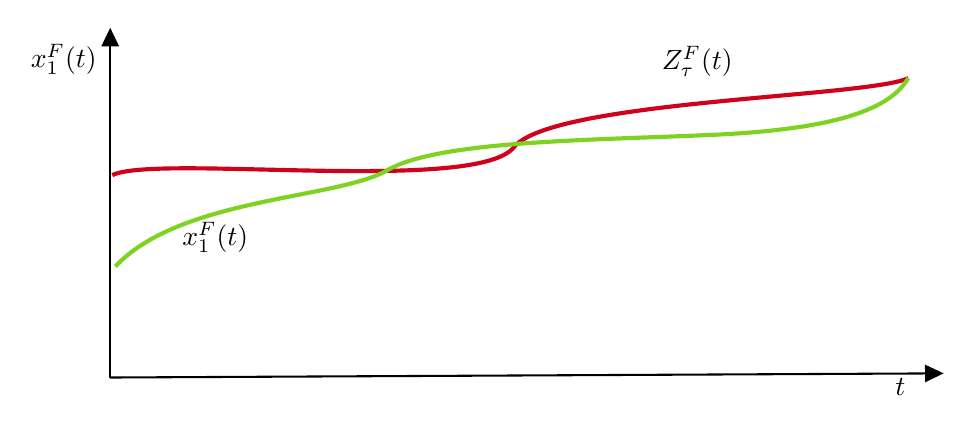
\begin{tikzpicture}[x=0.75pt,y=0.75pt,yscale=-1,xscale=1]
	%uncomment if require: \path (0,300); %set diagram left start at 0, and has height of 300
	
	%Curve Lines [id:da13273873192183094] 
	\draw [color={rgb, 255:red, 208; green, 2; blue, 27 }  ,draw opacity=1 ][line width=1.5]    (41.5,82.75) .. controls (62.66,72.39) and (217.06,91.85) .. (235,69.29) .. controls (252.94,46.73) and (406.16,45.22) .. (425,35.99) ;
	%Curve Lines [id:da36265400331191766] 
	\draw [color={rgb, 255:red, 126; green, 211; blue, 33 }  ,draw opacity=1 ][line width=1.5]    (43,126.75) .. controls (74,93.46) and (149.94,94.37) .. (174,80.38) .. controls (198.06,66.38) and (268,66.02) .. (329,63.41) .. controls (390,60.8) and (416.31,51.01) .. (425,35.99) ;
	%Straight Lines [id:da7392955293030656] 
	\draw [line width=0.75]    (40.5,180.25) -- (439,178.26) ;
	\draw [shift={(442,178.25)}, rotate = 179.71] [fill={rgb, 255:red, 0; green, 0; blue, 0 }  ][line width=0.08]  [draw opacity=0] (8.93,-4.29) -- (0,0) -- (8.93,4.29) -- cycle    ;
	%Straight Lines [id:da9916362390165014] 
	\draw [line width=0.75]    (40.5,180.25) -- (40.5,14.75) ;
	\draw [shift={(40.5,11.75)}, rotate = 90] [fill={rgb, 255:red, 0; green, 0; blue, 0 }  ][line width=0.08]  [draw opacity=0] (8.93,-4.29) -- (0,0) -- (8.93,4.29) -- cycle    ;
	
	% Text Node
	\draw (417.5,179.47) node [anchor=north west][inner sep=0.75pt]    {$t$};
	% Text Node
	\draw (1,18.4) node [anchor=north west][inner sep=0.75pt]    {$x_{1}^{F}( t)$};
	% Text Node
	\draw (74,104.3) node [anchor=north west][inner sep=0.75pt]    {$x_{1}^{F}( t)$};
	% Text Node
	\draw (305,19.34) node [anchor=north west][inner sep=0.75pt]    {$Z_{\tau }^{F}( t)$};
	
	
\end{tikzpicture}}
	\caption{Representation of $Z_{\tau}^\mathrm{F}$.}
	\label{fig:Z_tau}
\end{figure}
Figure~\ref{fig:Z_tau} illustrates the state space \(Z_{\tau}^{\mathrm{F}}(t)\) alongside time. This visualization is critical for understanding the operational scenario, especially under conditions where \(Z_{\tau}^{\mathrm{F}}(t)=0\). In this situation, if the Leader initiate to brake suddenly the Safety Barrier, which actuates the Emergency Braking, will not be intercepted before a period time of $\tau$ has passed, if no new update are received during the period $\left[t_0, t_0+\tau\right]$. Conversely, for conditions where \(Z_{\tau}^{\mathrm{F}}(t)>0\), the Safety Barrier's activation occurs prior to the lapse of $\tau$, whereas for \(Z_{\tau}^{\mathrm{F}}(t)<0\), activation is delayed, occurring after the period $\tau$.

This methodology plays a crucial role in reducing the intervention of the \gls{ecd} and, consequently, the frequency of emergency braking activations. Specifically, by choosing \(\hat{\tau}\), which, for instance, encapsulates 80\% of the communication intervals as delineated by Eq.~\eqref{eq:pdfDelay}, and setting \(\tau = \hat{\tau}\), we ensure that in 80\% of scenarios, the timing of communications suffices to preempt the activation of the Collision Detector. This is because, within this interval, the \gls{ecd} receives updated information from the Leader, effectively mitigating the likelihood of unnecessary emergency braking activation.

The \gls{h-nmpc} controller, illustrated in Figure \ref{fig:h-nmpc}, represents a hybrid architectural evolution of the model previously described. 
%
\begin{figure}[H]
	\resizebox{\linewidth}{!}{


\tikzset{every picture/.style={line width=0.75pt}} %set default line width to 0.75pt        

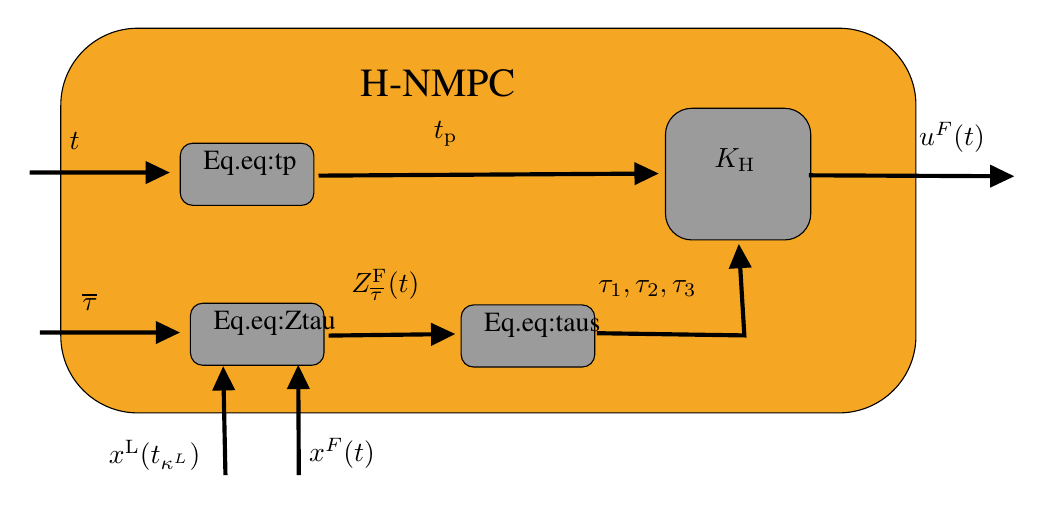
\begin{tikzpicture}[x=0.75pt,y=0.75pt,yscale=-1,xscale=1]
	%uncomment if require: \path (0,300); %set diagram left start at 0, and has height of 300
	
	%Rounded Rect [id:dp5342092506317702] 
	\draw  [fill={rgb, 255:red, 245; green, 166; blue, 35 }  ,fill opacity=1 ] (49,74.07) .. controls (49,53.6) and (65.6,37) .. (86.07,37) -- (423.93,37) .. controls (444.4,37) and (461,53.6) .. (461,74.07) -- (461,185.27) .. controls (461,205.74) and (444.4,222.33) .. (423.93,222.33) -- (86.07,222.33) .. controls (65.6,222.33) and (49,205.74) .. (49,185.27) -- cycle ;
	%Straight Lines [id:da7712511750690696] 
	\draw [line width=1.5]    (34.04,106.53) -- (97.47,106.54) ;
	\draw [shift={(101.47,106.54)}, rotate = 180.01] [fill={rgb, 255:red, 0; green, 0; blue, 0 }  ][line width=0.08]  [draw opacity=0] (11.61,-5.58) -- (0,0) -- (11.61,5.58) -- cycle    ;
	%Rounded Rect [id:dp43124631139892844] 
	\draw  [fill={rgb, 255:red, 155; green, 155; blue, 155 }  ,fill opacity=1 ] (340.33,88.25) .. controls (340.33,81.25) and (346.01,75.57) .. (353.02,75.57) -- (397.65,75.57) .. controls (404.65,75.57) and (410.33,81.25) .. (410.33,88.25) -- (410.33,126.31) .. controls (410.33,133.32) and (404.65,139) .. (397.65,139) -- (353.02,139) .. controls (346.01,139) and (340.33,133.32) .. (340.33,126.31) -- cycle ;
	
	%Rounded Rect [id:dp5272606094836356] 
	\draw  [fill={rgb, 255:red, 155; green, 155; blue, 155 }  ,fill opacity=1 ] (106.57,98.4) .. controls (106.57,95.1) and (109.25,92.42) .. (112.55,92.42) -- (164.94,92.42) .. controls (168.24,92.42) and (170.92,95.1) .. (170.92,98.4) -- (170.92,116.35) .. controls (170.92,119.65) and (168.24,122.33) .. (164.94,122.33) -- (112.55,122.33) .. controls (109.25,122.33) and (106.57,119.65) .. (106.57,116.35) -- cycle ;
	%Straight Lines [id:da3418278712403835] 
	\draw [line width=1.5]    (173.16,108.02) -- (333,107.03) ;
	\draw [shift={(337,107)}, rotate = 179.64] [fill={rgb, 255:red, 0; green, 0; blue, 0 }  ][line width=0.08]  [draw opacity=0] (11.61,-5.58) -- (0,0) -- (11.61,5.58) -- cycle    ;
	%Straight Lines [id:da20418654626243615] 
	\draw [line width=1.5]    (38.93,183.6) -- (102.36,183.61) ;
	\draw [shift={(106.36,183.61)}, rotate = 180.01] [fill={rgb, 255:red, 0; green, 0; blue, 0 }  ][line width=0.08]  [draw opacity=0] (11.61,-5.58) -- (0,0) -- (11.61,5.58) -- cycle    ;
	%Rounded Rect [id:dp15497890320530883] 
	\draw  [fill={rgb, 255:red, 155; green, 155; blue, 155 }  ,fill opacity=1 ] (111.46,175.47) .. controls (111.46,172.17) and (114.14,169.49) .. (117.45,169.49) -- (169.83,169.49) .. controls (173.14,169.49) and (175.81,172.17) .. (175.81,175.47) -- (175.81,193.42) .. controls (175.81,196.72) and (173.14,199.4) .. (169.83,199.4) -- (117.45,199.4) .. controls (114.14,199.4) and (111.46,196.72) .. (111.46,193.42) -- cycle ;
	%Straight Lines [id:da9062761049292425] 
	\draw [line width=1.5]    (178.05,185.09) -- (235,184.38) ;
	\draw [shift={(239,184.33)}, rotate = 179.29] [fill={rgb, 255:red, 0; green, 0; blue, 0 }  ][line width=0.08]  [draw opacity=0] (11.61,-5.58) -- (0,0) -- (11.61,5.58) -- cycle    ;
	%Straight Lines [id:da3679270230297198] 
	\draw [line width=1.5]    (128.33,252.33) -- (127.33,203.9) ;
	\draw [shift={(127.25,199.9)}, rotate = 88.81] [fill={rgb, 255:red, 0; green, 0; blue, 0 }  ][line width=0.08]  [draw opacity=0] (11.61,-5.58) -- (0,0) -- (11.61,5.58) -- cycle    ;
	%Straight Lines [id:da12861115805060974] 
	\draw [line width=1.5]    (163.67,252.33) -- (163.42,203.23) ;
	\draw [shift={(163.4,199.23)}, rotate = 89.72] [fill={rgb, 255:red, 0; green, 0; blue, 0 }  ][line width=0.08]  [draw opacity=0] (11.61,-5.58) -- (0,0) -- (11.61,5.58) -- cycle    ;
	%Rounded Rect [id:dp8841367496827979] 
	\draw  [fill={rgb, 255:red, 155; green, 155; blue, 155 }  ,fill opacity=1 ] (241.89,176.3) .. controls (241.89,172.99) and (244.56,170.32) .. (247.87,170.32) -- (300.25,170.32) .. controls (303.56,170.32) and (306.24,172.99) .. (306.24,176.3) -- (306.24,194.25) .. controls (306.24,197.55) and (303.56,200.23) .. (300.25,200.23) -- (247.87,200.23) .. controls (244.56,200.23) and (241.89,197.55) .. (241.89,194.25) -- cycle ;
	%Straight Lines [id:da6141145674275619] 
	\draw [line width=1.5]    (307.25,183.93) -- (378.33,185) -- (375.91,144.99) ;
	\draw [shift={(375.67,141)}, rotate = 86.53] [fill={rgb, 255:red, 0; green, 0; blue, 0 }  ][line width=0.08]  [draw opacity=0] (11.61,-5.58) -- (0,0) -- (11.61,5.58) -- cycle    ;
	%Straight Lines [id:da36494876539861076] 
	\draw [line width=1.5]    (409.37,107.86) -- (504.33,108.31) ;
	\draw [shift={(508.33,108.33)}, rotate = 180.27] [fill={rgb, 255:red, 0; green, 0; blue, 0 }  ][line width=0.08]  [draw opacity=0] (11.61,-5.58) -- (0,0) -- (11.61,5.58) -- cycle    ;
	
	
	% Text Node
	\draw (306.74,157.15) node [anchor=north west][inner sep=0.75pt]    {$\tau _{1} ,\tau _{2} ,\tau _{3}$};
	% Text Node
	\draw (251.75,173.02) node [anchor=north west][inner sep=0.75pt]   [align=left] {{\fontfamily{ptm}\selectfont Eq.\eqref{eq:taus}}};
	% Text Node
	\draw (70.93,234.37) node [anchor=north west][inner sep=0.75pt]    {$x^{\mathrm{L}}( t_{\kappa ^{L}})$};
	% Text Node
	\draw (167.41,233.41) node [anchor=north west][inner sep=0.75pt]    {$x^{F}( t)$};
	% Text Node
	\draw (187.69,151.89) node [anchor=north west][inner sep=0.75pt]    {$Z_{\overline{\tau }}^{\mathrm{F}}( t)$};
	% Text Node
	\draw (121.33,172.2) node [anchor=north west][inner sep=0.75pt]   [align=left] {{\fontfamily{ptm}\selectfont Eq.\eqref{eq:Ztau}}};
	% Text Node
	\draw (58.07,163.47) node [anchor=north west][inner sep=0.75pt]    {$\overline{\tau }$};
	% Text Node
	\draw (227.47,80.82) node [anchor=north west][inner sep=0.75pt]    {$t_{\mathrm{p}}$};
	% Text Node
	\draw (116.43,95.13) node [anchor=north west][inner sep=0.75pt]   [align=left] {{\fontfamily{ptm}\selectfont Eq.\eqref{eq:tp}}};
	% Text Node
	\draw (51.99,85.91) node [anchor=north west][inner sep=0.75pt]    {$t$};
	% Text Node
	\draw (461.33,81.07) node [anchor=north west][inner sep=0.75pt]    {$u^{F}( t)$};
	% Text Node
	\draw (192,55.67) node [anchor=north west][inner sep=0.75pt]  [font=\Large] [align=left] {{\fontfamily{ptm}\selectfont H-NMPC}};
	% Text Node
	\draw (362.67,93.7) node [anchor=north west][inner sep=0.75pt]    {$K_{\mathrm{H}}$ };
	
	
\end{tikzpicture}}
	\caption{Control system architecture for \gls{vc} operation. Blue and orange boxes are communication and control modules, respectively. }
	\label{fig:h-nmpc}
\end{figure}
%
The controller $K_{\tau_j}$ is defined based on a specified state region $Z_{\tau_j}\left(\underline{x}^\mathrm{L}(t),\hat{x}^\mathrm{F}(t)\right)$, where the subscript $\tau_j \in \{\tau_1,\tau_2,\tau_3\}$, ensuring that
\begin{equation*}
	\tau_1 \leq \tau_2 \leq \tau_3, \quad \text{and} \quad H>\tau_3.
\end{equation*}
For this particular application, the timing parameters are selected as follows
\begin{equation*}
	\tau_1 = \frac{1}{3}\hat{\tau}, \quad
	\tau_2 = \frac{2}{3}\hat{\tau}, \quad
	\tau_3 = \hat{\tau},
\end{equation*}
different values could be selected based on the specific requirements or objectives of the application.

%
\begin{figure}[H]
	\resizebox{\linewidth}{!}{


\tikzset{every picture/.style={line width=0.75pt}} %set default line width to 0.75pt        

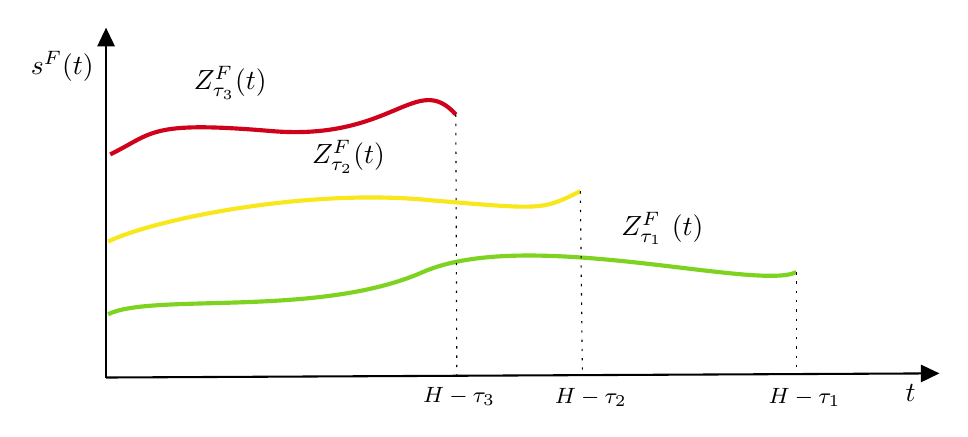
\begin{tikzpicture}[x=0.75pt,y=0.75pt,yscale=-1,xscale=1]
	%uncomment if require: \path (0,300); %set diagram left start at 0, and has height of 300
	
	%Curve Lines [id:da3576386679434109] 
	\draw [color={rgb, 255:red, 126; green, 211; blue, 33 }  ,draw opacity=1 ][line width=1.5]    (41.5,149.75) .. controls (62.66,139.39) and (143,151.5) .. (193,129.5) .. controls (243,107.5) and (354.16,138.73) .. (373,129.5) ;
	%Straight Lines [id:da044701537193025276] 
	\draw [line width=0.75]    (40.5,180.25) -- (439,178.26) ;
	\draw [shift={(442,178.25)}, rotate = 179.71] [fill={rgb, 255:red, 0; green, 0; blue, 0 }  ][line width=0.08]  [draw opacity=0] (8.93,-4.29) -- (0,0) -- (8.93,4.29) -- cycle    ;
	%Straight Lines [id:da0008580645658053943] 
	\draw [line width=0.75]    (40.5,180.25) -- (40.5,14.75) ;
	\draw [shift={(40.5,11.75)}, rotate = 90] [fill={rgb, 255:red, 0; green, 0; blue, 0 }  ][line width=0.08]  [draw opacity=0] (8.93,-4.29) -- (0,0) -- (8.93,4.29) -- cycle    ;
	%Curve Lines [id:da6528039000875612] 
	\draw [color={rgb, 255:red, 248; green, 231; blue, 28 }  ,draw opacity=1 ][line width=1.5]    (41.5,114.75) .. controls (62.66,104.39) and (134,89.5) .. (193,94.5) .. controls (252,99.5) and (250.16,99.73) .. (269,90.5) ;
	%Curve Lines [id:da6773052220718958] 
	\draw [color={rgb, 255:red, 208; green, 2; blue, 27 }  ,draw opacity=1 ][line width=1.5]    (42.5,72.75) .. controls (63.66,62.39) and (61,56.5) .. (120,61.5) .. controls (179,66.5) and (190,32.5) .. (209,53.5) ;
	%Straight Lines [id:da36906188743755486] 
	\draw  [dash pattern={on 0.84pt off 2.51pt}]  (209,53.5) -- (209.5,179.75) ;
	%Straight Lines [id:da5037794242478335] 
	\draw  [dash pattern={on 0.84pt off 2.51pt}]  (269,90.5) -- (270,179.25) ;
	%Straight Lines [id:da2541577667107384] 
	\draw  [dash pattern={on 0.84pt off 2.51pt}]  (373,129.5) -- (373,179.25) ;
	
	% Text Node
	\draw (424.5,182.37) node [anchor=north west][inner sep=0.75pt]    {$t$};
	% Text Node
	\draw (3,21.8) node [anchor=north west][inner sep=0.75pt]    {$s^{F}( t)$};
	% Text Node
	\draw (81.5,29.24) node [anchor=north west][inner sep=0.75pt]    {$Z_{\tau _{3}}^{F}( t)$};
	% Text Node
	\draw (138.5,64.74) node [anchor=north west][inner sep=0.75pt]    {$Z_{\tau _{2}}^{F}( t)$};
	% Text Node
	\draw (287.5,99.24) node [anchor=north west][inner sep=0.75pt]    {$Z_{\tau _{1\ }}^{F}( t)$};
	% Text Node
	\draw (358.5,184.37) node [anchor=north west][inner sep=0.75pt]  [font=\footnotesize]  {$H-\tau _{1}$};
	% Text Node
	\draw (255.5,184.37) node [anchor=north west][inner sep=0.75pt]  [font=\footnotesize]  {$H-\tau _{2}$};
	% Text Node
	\draw (192,183.87) node [anchor=north west][inner sep=0.75pt]  [font=\footnotesize]  {$H-\tau _{3}$};
	
	
\end{tikzpicture}}
	\caption{Control system architecture for \gls{vc} operation. Blue and orange boxes are communication and control modules, respectively. }
	\label{fig:Z_tau_graph}
\end{figure}

Figure \ref{fig:Z_tau_graph} shows the state spaces considered by the control system; specifically, since the $Z_{\tau_j}$ function is monotonically increasing, we have that for ever larger values of $\tau_j$, the various $Z_{\tau_j}$ curves have a greater value.  Depending on the Follower's position, it will be situated within a region of the space delineated by the curves $Z_{\tau_j}$. Based on the state space under consideration, we will differentiate between three types of controllers as reported in Figure\tildeAdd\ref{fig:controlSystem}. In the following discussion on controllers, we will focus exclusively on the cost functions. It's important to note that the constraints associated with the optimization problem of the \gls{nmpc} remain consistent with those detailed in Eqs.\eqref{eq:t-nmpc}.

The first controller, $K_{\tau_{1}}$, designated as the \gls{l3}-\gls{vc} coupling controller when $Z_{\tau_1} < 0$, is implemented for the safest state space. The optimization problem it aims to solve is outlined as follows
%
\begin{equation}
	\min_{u_{\tau_{1}}^F(t)} \int_{t}^{t+H} L_{Q_{\tau_1}}(Z_{\tau_1}(r),u_{\tau_{1}}^F(r)) dr + L_{H_{\tau_{1}}}(Z_{\tau_1}(H)),
\end{equation}
%
where
\begin{align*}
	&L_{H_{\tau_{1}}}(Z_{\tau_1}(H)) =  Z_{\tau_1}\left(\underline{x}^\mathrm{L}(H),\hat{x}^\mathrm{F}(H)\right) Q_{H_{\tau_1}} Z_{\tau_1}\left(\underline{x}^\mathrm{L}(H),\hat{x}^\mathrm{F}(H)\right), \\
	&L_{Q_{\tau_1}}(Z_{\tau_1}(r),u_{\tau_{1}}^F(r)) =  u_{\tau_{1}}^F(r)  Q_u u_{\tau_{1}}^F(r) \\
	&\quad +  Z_{\tau_1}\left(\underline{x}^\mathrm{L}(r),\hat{x}^\mathrm{F}(r)\right) Q_{\tau_1} Z_{\tau_1}\left(\underline{x}^\mathrm{L}(r),\hat{x}^\mathrm{F}(r)\right).
\end{align*}
\blue{specifiy the cost function properties.}

The controller $K_{\tau_{2}}$ is tasked with supporting the \gls{vc} under normal operating conditions. Its functional cost is defined as follows
%
\begin{equation}
	\min_{u_{\tau_{2}}^F(t)} \int_{t}^{t+H} L_{Q_{\tau_2}}(Z_{\tau_2}(r),u_{\tau_{2}}^F(r)) dr + L_{H_{\tau_{2}}}(Z_{\tau_2}(H)).
\end{equation}
%
where
\begin{align*}
	&L_{H_{\tau_{2}}}(Z_{\tau_2}(H)) =  Z_{\tau_2}\left(\underline{x}^\mathrm{L}(H),\hat{x}^\mathrm{F}(H)\right) Q_{H_{\tau_2}} Z_{\tau_2}\left(\underline{x}^\mathrm{L}(H),\hat{x}^\mathrm{F}(H)\right), \\
	&L_{Q_{\tau_2}}(Z_{\tau_2}(r),u_{\tau_{2}}^F(r)) =  Z_{\tau_2}\left(\underline{x}^\mathrm{L}(r),\hat{x}^\mathrm{F}(r)\right) Q_{\tau_2} Z_{\tau_2}\left(\underline{x}^\mathrm{L}(r),\hat{x}^\mathrm{F}(r)\right)  \\
	& \quad \quad  + u_{\tau_{2}}^F(r)  Q_u u_{\tau_{2}}^F(r) + (\hat{x}_2^F(r)-v_{\textit{ave}}^\mathrm{L}) Q_{v} (\hat{x}_2^F(r)-v_{\textit{ave}}^\mathrm{L}).
\end{align*}
\blue{specifiy the cost function properties.}

The final controller, $K_{\tau_{3}}$, is deployed in scenarios where the \gls{vc} approaches critical conditions. Its cost function is defined as follows
%
\begin{equation}
	\min_{u_{\tau_{3}}^F(t)} \int_{t}^{t+H} L_{Q_{\tau_3}}(Z_{\tau_2}(r),Z_{\tau_3}(r),u_{\tau_{3}}^F(r)) dr + L_{H_{\tau_{3}}}(Z_{\tau_3}(H)),
\end{equation}
%
where
\begin{align*}
	&L_{H_{\tau_{1}}}(Z_{\tau_1}(H)) =  Z_{\tau_1}\left(\underline{x}^\mathrm{L}(H),\hat{x}^\mathrm{F}(H)\right) Q_{H_{\tau_1}} Z_{\tau_1}\left(\underline{x}^\mathrm{L}(H),\hat{x}^\mathrm{F}(H)\right), \\
	&L_{Q_{\tau_3}}(Z_{\tau_2}(r),Z_{\tau_3}(r),u_{\tau_{3}}^F(r)) =  u_{\tau_{3}}^F(r)  Q_u u_{\tau_{3}}^F(r)  \\
	&\quad +  Z_{\tau_3}\left(\underline{x}^\mathrm{L}(r),\hat{x}^\mathrm{F}(r)\right) Q_{\tau_3} Z_{\tau_3}\left(\underline{x}^\mathrm{L}(r),\hat{x}^\mathrm{F}(r)\right) \\
	&\quad + Z_{\tau_2}\left(\underline{x}^\mathrm{L}(r),\hat{x}^\mathrm{F}(r)\right) Q_{\tau_2} Z_{\tau_2}\left(\underline{x}^\mathrm{L}(r),\hat{x}^\mathrm{F}(r)\right).
\end{align*}
\blue{specifiy the cost function properties.}

In scenarios such as \ref{enum:channel2}, characterized by communication delays and packet losses, the adjustments to the control architecture are minimal. Each communication packet is augmented with a timestamp to manage delays effectively. Consider a situation where the Leader dispatches the current packet at time $\ell_{\kappa^\mathcal{L}}(t)$, and the Follower receives it at $\ell_{\kappa^\mathcal{LF}}(t)$, where $\ell_{\kappa^\mathcal{LF}}(t) > \ell_{\kappa^\mathcal{L}}(t)$. The\gls{ecd}'s predictor is initialized at $\ell_{\kappa^\mathcal{L}}(t)$ and used from $\ell_{\kappa^\mathcal{LF}}(t)$. Similarly, computations for $Z_{\tau_j}^{\mathcal{F}}(t)$ commence from $\ell_{\kappa^\mathcal{L}}(t)$ but are applicable from $\ell_{\kappa^\mathcal{LF}}(t)$ onwards. It is imperative to select a prediction horizon $H$ that exceeds $\tau_3 + \Delta$, with $\Delta$ representing the upper limit of delays, to ensure robust performance. Beyond this adjustment, the process mirrors the approach outlined for the scenario \ref{enum:channel1}, demonstrating the architecture's adaptability to varied communication conditions.










%
%%% END SECTION ============================================================
%%% START SECTION ==========================================================
\section{Simulations}
\label{sec:Simulations}

\blue{TODO}



%%% END SECTION ============================================================
%%% START SECTION ==========================================================
\section{Conclusion}
\label{sec:conclusion}

\blue{TODO}


\appendix

\subsection{Proof of Lemma \ref{lemma:Proxies}}
\label{appendix:proxy}


Firstly, let us consider the inequality stated in \eqref{lemma:rlpProxy}. For the demonstration, we will calculate the following differential equations
\begin{align*}
	\dot{\tilde{x}}^i = \overline{f}\left(\tilde{x}^i, u^i \right) - f\left(\tilde{x}^i, u^i, p^i \right), \\
	\dot{\hat{x}}^i = f\left(\hat{x}^i, u^i \right) - \underline{f}\left(\hat{x}^i, u^i, p^i \right),
\end{align*}
for the sake of brevity in calculations, we will directly show the result
\begin{equation}
	\label{eq:lemmarup}
	\begin{cases}
		\dot{\tilde{x}}_1^i =   0, \qquad  \qquad \qquad \qquad \qquad \qquad  \qquad  \text{if} \; u^i < 0,  \\
		\dot{\tilde{x}}_2^i = \frac{A^i \overline{M}^i - \underline{A}^i M^i}{M^i \overline{M}^i} + B^i \tilde{x}_2^i + T_f^i C^i \left(\tilde{x}_2^i\right)^2+ \left(F_e - \underline{F}_e\right) \\ \noalign{\vskip3pt} \quad \; \;\  + \frac{M^i-\underline{M}^i}{M^i \underline{M}^i}u^i, \\ 
		\noalign{\vskip9pt}
		\dot{\tilde{x}}_1^i =   0, \qquad  \qquad \qquad \qquad \qquad \qquad  \qquad  \text{if} \; u^i \geq 0,  \\
		\dot{\tilde{x}}_2^i = \frac{Ai \overline{M}^i - \underline{A}^i M^i}{M^i \overline{M}^i} + \frac{B^i \overline{M}^i - \underline{B}^i M^i}{M^i \overline{M}^i} \tilde{x}_2^i + \frac{T_f^i C^i \overline{M}^i - \underline{T}_f^i\underline{C}^i M^i}{M^i \overline{M}^i}  \left(\tilde{x}_2^i\right)^2 \\  
		\noalign{\vskip3pt} \quad \; \;\ + \frac{M^i-\underline{M}^i}{M^i \underline{M}^i}u^i. \\ 
	\end{cases}
\end{equation}
and 
\begin{equation}
	\label{eq:lemmarlp}
	\begin{cases}
		\dot{\hat{x}}_1^i =   0, \qquad  \qquad \qquad \qquad \qquad \qquad  \qquad  \text{if} \; u^i < 0,  \\
		\frac{ \overline{A}^i M^i - \underline{M}^i A^i}{M^i \underline{M}^i} + \frac{M^i \overline{B}^i - \underline{M}^i B^i}{M^i \underline{M}^i} \hat{x}_2^i + \frac{M^i  \overline{T_f}^i \overline{C}^i -  \underline{M}^i T_f^i C^i}{M^i \underline{M}^i}  \left(\hat{x}_2^i\right)^2 \\  
		\noalign{\vskip3pt} \quad \; \;\ + \frac{\overline{M}^i - M^i}{M^i \overline{M}^i}u^i, \\ 
		\noalign{\vskip9pt}
		\dot{\hat{x}}_1^i =   0, \qquad  \qquad \qquad \qquad \qquad \qquad  \qquad  \text{if} \; u^i \geq 0,  \\
		\dot{\hat{x}}_2^i = \frac{ \overline{A}^i M^i - \underline{M}^i A^i}{M^i \underline{M}^i} + \frac{M^i \overline{B}^i - \underline{M}^i B^i}{M^i \underline{M}^i} \hat{x}_2^i + \frac{M^i  \overline{T_f}^i \overline{C}^i -  \underline{M}^i T_f^i C^i}{M^i \underline{M}^i}  \left(\hat{x}_2^i\right)^2 \\  
		\noalign{\vskip3pt} \quad \; \;\ + (\overline{F}^i_e - {F}^i_e) + \frac{\overline{M}^i - M^i}{M^i \overline{M}^i}u^i. \\ 
	\end{cases}
\end{equation}
%
Given the systems defined in Eq.\eqref{eq:lemmarup} and Eq.\eqref{eq:lemmarlp}, all component terms are observed to be non-negative. This ensures the system's positivity, facilitating the derivation of the following equations that supports the lemma.

\subsection{Proof of Theorem \ref{theom:Safety}}
\label{appendix:Safety}

We first consider affine control systems version of model \ref{eq:robustModel} expressed as
%
\begin{equation} \label{eq:affine}
	\dot{x} =  \begin{bmatrix}
		\dot{x}^L_{1} \\
		\dot{x}^L_{2} \\
		\dot{x}^F_{1} \\
		\dot{x}^F_{2}
	\end{bmatrix} = f(x) + g(x)u,
\end{equation}
%
where $x= \left[x_1^L \; x_2^L \; x_1^F \; x_2^F\right]$, $u=K_{\mathrm{E}}\left({x}^{\mathrm{F}}\right)$ and
\begin{equation}
	f(x) = \begin{bmatrix}
		x^L_{2} \\
		\frac{1}{M^L}(-A^L-B^L x_2^L - T_\mathrm{F}^L C^L (x_2^L)^2)-\mathrm{F}_e^L +K\left({x}^{\mathrm{L}} \right) \\
		x^F_{2} \\
		\frac{1}{M^F}(-A^F-B^F x_2^F - T_\mathrm{F}^F C^F (x_2^F)^2)-\mathrm{F}_e^F \\
	\end{bmatrix},
\end{equation}
\begin{equation}
	g(x) = \begin{bmatrix}
		0 \\
		0 \\
		0 \\
		\frac{1}{M^F}
	\end{bmatrix}.
\end{equation}
At this point, we calculate the condition \eqref{eq:barrierCertificate} for the  first  of the two barrier functions, $B'(x)$, which satisfies \eqref{eq:barrierNegative} and leads to
%
\begin{equation}
	u' \leq -\frac{L_f B'(x)}{L_g B'(x)}.
\end{equation}
%
For the second barrier function $B''(x)$ we notice that $L_g B''(x) = 0$ for \eqref{eq:barrierCertificate} thus the control input
$u$ does not show up, thus we cannot use this
barrier function but we must use the notion of High Order Barrier Function (HOBF). Since $B''(x)$ is a $2^{\text{th}}$ order differentiable
function we define the following functions
%
\begin{equation} \label{eq:psi}
	\begin{aligned}
		& \psi_0(x):=B''(x) \\
		& \psi_1(x):=\dot{\psi}_0(x)+\epsilon \psi_0(x), \\
		& \psi_2(x):=\dot{\psi}_1(x)+\epsilon \psi_1(x),
	\end{aligned}
\end{equation}
%
where $\epsilon > 0$ denote a constant used as linear class $\mathcal{K}$ function.

We further define the sets $S_{\psi_1}$ and $ S_{\psi_2} $ associated with \eqref{eq:psi} in the form
%
\begin{align} \
	S_{\psi_1} =\left\{{x} \in \mathbb{R}^n: \psi_0({x}) \geq 0\right\}, \\
	S_{\psi_2} =\left\{{x} \in \mathbb{R}^n: \psi_1({x}) \geq 0\right\}.
\end{align}
%
The function $B''(x)$ is a High Order Control Barrier Function (HOCBF) of degree 2 for system \eqref{eq:affine} thus satisfies
%
\begin{equation}
	L_f^2 B''(x)+L_g L_f B''(x) u'' \\
	+\epsilon\left(\psi_{1}(x)\right) \leq 0
\end{equation}
Hence we obtain the condition for $u''$ as
\begin{equation}
	u'' \leq - \frac{L_f^2 B''(x)+\epsilon\left(\psi_{1}(x)\right)}{L_g L_f B''(x)}
\end{equation}

In order for the following inequality $\dot{B}\left(x^\mathrm{L}\left(t\right),x^\mathrm{F}\left(t\right)\right) \leq 0$ to be verified, it would be necessary that the following condition  is satisfied

\begin{equation}
	u=K_{\mathrm{E}}\left({x}^{\mathrm{F}}\right) = \min\left\{u',u''\right\}.
\end{equation}